\documentclass[10pt,journal,compsoc]{IEEEtran}
%
% If IEEEtran.cls has not been installed into the LaTeX system files,
% manually specify the path to it like:
% \documentclass[journal,comsoc]{../sty/IEEEtran}


%%%%%%%%%%%%%%%%%%%%%%%%%%%%%%%%%%%%%%%%%%%%%%%%%%%%%%%%%%%%%
%% copied from thesis
%%%%%%%%%%%%%%%%%%%%%%%%%%%%%%%%%%%%%%%%%%%%%%%%%%%%%%%%%%%%%
%% Packages für Formeln %%%%%%%%%%%%%%%%%%%%%%%%%%%%%%%%%%%%%
\usepackage[colorlinks,
            linkcolor=red,
            anchorcolor=blue,
            citecolor=green
            ]{hyperref}
\usepackage{amsmath}
\usepackage{amsthm}
%\usepackage{amsfonts}
\usepackage{amssymb}
\usepackage{booktabs}
\newcommand{\ra}[1]{\renewcommand{\arraystretch}{#1}}

%% Packages
%\usepackage{tikz}
%\usetikzlibrary{shapes,arrows}
%\usetikzlibrary{positioning}
\usepackage{graphicx}
\usepackage{kantlipsum} %<- For dummy text
\usepackage{mwe} %<- For dummy images
\usepackage{multirow}
\usepackage{multicol}
%\usepackage{colortbl}
%\usepackage{todonotes}	
\newcounter{todocounter}
\newcommand{\todonum}[2][]
{\stepcounter{todocounter}\todo[inline,backgroundcolor=blue!10!white, #1]{\thetodocounter: #2}}

%% Zeilenabstand %%%%%%%%%%%%%%%%%%%%%%%%%%%%%%%%%%%%%%%%%%%%
\usepackage{setspace}
%\singlespacing        %% 1-zeilig (Standard)
%\onehalfspacing       %% 1,5-zeilig
%\doublespacing        %% 2-zeilig


%% Andere Packages %%%%%%%%%%%%%%%%%%%%%%%%%%%%%%%%%%%%%%%%%%
%\usepackage{a4wide} %%Kleinere Seitenränder = mehr Text pro Zeile.
\usepackage{fancyhdr} %%Fancy Kopf- und Fußzeilen
%\usepackage{longtable} %%Für Tabellen, die eine Seite überschreiten
\usepackage{lscape}
\usepackage{rotating} 
%\usepackage[htt]{hyphenat} %Trennung von Typewriter-Schriften
%\usepackage{listings}
%\usepackage{pstricks-add} --> This package generates problems with booktabs (toprule, etc.)
\usepackage[autostyle]{csquotes}
\usepackage{amsmath,bm}
\usepackage{array}
% Tabellen mit Center und left
\usepackage{tabularx,colortbl} % colored table background
\newcolumntype{C}[1]{>{\centering\arraybackslash}p{#1}}
\newcolumntype{R}[1]{>{\raggedleft\arraybackslash}p{#1}}
\newcolumntype{L}[1]{>{\raggedright\arraybackslash}p{#1}}
% Table spacings
\newcommand\T{\rule{0pt}{2.5ex}\rule[-1.0ex]{0pt}{0pt}}
\newcommand\B{\rule[-1.0ex]{0pt}{0pt}}

\definecolor{slightgray}{gray}{.90} 
\usepackage{rotating}
\usepackage{hhline}



\newtheoremstyle{mytheoremstyle} % name
        {\topsep}                    % Space above
        {\topsep}                    % Space below
        {\itshape\fontfamily{ptm}\selectfont}                   % Body font, ptm is times new roma
        {}                           % Indent amount
        {\fontfamily{ptm}\selectfont\scshape\color{black}\bfseries}                   % Theorem head font
        {:}                          % Punctuation after theorem head
        {.5em}                       % Space after theorem head
        {}  % Theorem head spec (can be left empty, meaning ‘normal’)

  
          
\theoremstyle{mytheoremstyle}
\newtheorem{theorem}{Theorem}[section]

\theoremstyle{mytheoremstyle}
\newtheorem{corollary}{Corollary}[section]

\theoremstyle{mytheoremstyle}
\newtheorem{lemma}{Lemma}[section]

%\theoremstyle{mytheoremstyle}
%\let\definition\relax
\newtheorem{mydef}{Definition}%[section]

%%%%%%
%%%%%% Proof
    \makeatletter
    \renewenvironment{proof}[1][\proofname]{%
      \par\pushQED{\qed}\fontfamily{ptm}\selectfont%
      \topsep6\p@\@plus6\p@\relax
      \trivlist\item[\hskip\labelsep\bfseries#1\@addpunct{.}]%
      \ignorespaces
    }{%
      \popQED\endtrivlist\@endpefalse
    }
    \makeatother 
%%%%%%%%%%%%%%%%%

\newcommand{\eg}{e.g., }
\newcommand{\ie}{i.e., }
\usepackage[linesnumbered,ruled,vlined]{algorithm2e}
%\usepackage{algorithmic}
\usepackage{times}
%\usepackage{mathptmx}
\usepackage{mathtools}
\usepackage[draft,nomargin,marginclue,footnote,silent]{fixme}
\setcounter{tocdepth}{2}

\makeatother
\usepackage{comment}
\newcommand{\Tau}{\mathrm{T}}
\usepackage[colorinlistoftodos]{todonotes}
\DeclareMathOperator*{\Max}{Max}
\DeclareMathOperator*{\Min}{Min}

\newcommand{\bigO}{\ensuremath{\mathcal{O}}}% big-O notation/symbol
\usepackage{subfigure}
\usepackage{adjustbox}
\usepackage{multirow}
\usepackage{enumitem}
\usepackage{lipsum}
\setlist[itemize]{leftmargin=*}
%%%%%%%%%%%%%%%%%%%%%%%%%% copied from thesis
%%%%%%%%%%%%%%%%%%%%%%%%%%%


\usepackage[T1]{fontenc}% optional T1 font encoding



% *** GRAPHICS RELATED PACKAGES ***
%
\ifCLASSINFOpdf
  % \usepackage[pdftex]{graphicx}
  % declare the path(s) where your graphic files are
  % \graphicspath{{../pdf/}{../jpeg/}}
  % and their extensions so you won't have to specify these with
  % every instance of \includegraphics
  % \DeclareGraphicsExtensions{.pdf,.jpeg,.png}
\else
  % or other class option (dvipsone, dvipdf, if not using dvips). graphicx
  % will default to the driver specified in the system graphics.cfg if no
  % driver is specified.
  % \usepackage[dvips]{graphicx}
  % declare the path(s) where your graphic files are
  % \graphicspath{{../eps/}}
  % and their extensions so you won't have to specify these with
  % every instance of \includegraphics
  % \DeclareGraphicsExtensions{.eps}
\fi
% graphicx was written by David Carlisle and Sebastian Rahtz. It is
% required if you want graphics, photos, etc. graphicx.sty is already
% installed on most LaTeX systems. The latest version and documentation
% can be obtained at: 
% http://www.ctan.org/pkg/graphicx
% Another good source of documentation is "Using Imported Graphics in
% LaTeX2e" by Keith Reckdahl which can be found at:
% http://www.ctan.org/pkg/epslatex
%
% latex, and pdflatex in dvi mode, support graphics in encapsulated
% postscript (.eps) format. pdflatex in pdf mode supports graphics
% in .pdf, .jpeg, .png and .mps (metapost) formats. Users should ensure
% that all non-photo figures use a vector format (.eps, .pdf, .mps) and
% not a bitmapped formats (.jpeg, .png). The IEEE frowns on bitmapped formats
% which can result in "jaggedy"/blurry rendering of lines and letters as
% well as large increases in file sizes.
%
% You can find documentation about the pdfTeX application at:
% http://www.tug.org/applications/pdftex





% *** MATH PACKAGES ***
%
\usepackage{amsmath}
% A popular package from the American Mathematical Society that provides
% many useful and powerful commands for dealing with mathematics.
% Do NOT use the amsbsy package under comsoc mode as that feature is
% already built into the Times Math font (newtxmath, mathtime, etc.).
% 
% Also, note that the amsmath package sets \interdisplaylinepenalty to 10000
% thus preventing page breaks from occurring within multiline equations. Use:
\interdisplaylinepenalty=2500
% after loading amsmath to restore such page breaks as IEEEtran.cls normally
% does. amsmath.sty is already installed on most LaTeX systems. The latest
% version and documentation can be obtained at:
% http://www.ctan.org/pkg/amsmath


% Select a Times math font under comsoc mode or else one will automatically
% be selected for you at the document start. This is required as Communications
% Society journals use a Times, not Computer Modern, math font.
%\usepackage[cmintegrals]{newtxmath}
\usepackage{txfonts}
% The freely available newtxmath package was written by Michael Sharpe and
% provides a feature rich Times math font. The cmintegrals option, which is
% the default under IEEEtran, is needed to get the correct style integral
% symbols used in Communications Society journals. Version 1.451, July 28,
% 2015 or later is recommended. Also, do *not* load the newtxtext.sty package
% as doing so would alter the main text font.
% http://www.ctan.org/pkg/newtx
%
% Alternatively, you can use the MathTime commercial fonts if you have them
% installed on your system:
%\usepackage{mtpro2}
%\usepackage{mt11p}
%\usepackage{mathtime}


%\usepackage{bm}
% The bm.sty package was written by David Carlisle and Frank Mittelbach.
% This package provides a \bm{} to produce bold math symbols.
% http://www.ctan.org/pkg/bm


% correct bad hyphenation here
\hyphenation{op-tical net-works semi-conduc-tor}
\DeclareMathOperator*{\argmin}{arg\,min}
\DeclareMathOperator*{\argmax}{arg\,max}

\begin{document}
%
% paper title
% Titles are generally capitalized except for words such as a, an, and, as,
% at, but, by, for, in, nor, of, on, or, the, to and up, which are usually
% not capitalized unless they are the first or last word of the title.
% Linebreaks \\ can be used within to get better formatting as desired.
% Do not put math or special symbols in the title.
\title{Versatile Robust Clustering of Ad Hoc Cognitive Radio Network}
%
%
% author names and IEEE memberships
% note positions of commas and nonbreaking spaces ( ~ ) LaTeX will not break
% a structure at a ~ so this keeps an author's name from being broken across
% two lines.
% use \thanks{} to gain access to the first footnote area
% a separate \thanks must be used for each paragraph as LaTeX2e's \thanks
% was not built to handle multiple paragraphs
%

\author{Di~Li,~\IEEEmembership{Member,~IEEE,}
        Erwin~Fang,
        and James~Gross,~\IEEEmembership{Member,~IEEE}% <-this % stops a space
\thanks{D. Li was with RWTH Aachen university, Germany.}% <-this % stops a space
\thanks{Erwin. Fang is with ETH, Switzerland.}% <-this % stops a space
\thanks{J. Gross is with KTH Royal Institute of Technology, Sweden.}% <-this % stops a space
\thanks{Manuscript received xxxx xx, 20xx; revised xxxx xx, 20xx.}}

% note the % following the last \IEEEmembership and also \thanks - 
% these prevent an unwanted space from occurring between the last author name
% and the end of the author line. i.e., if you had this:
% 
% \author{....lastname \thanks{...} \thanks{...} }
%                     ^------------^------------^----Do not want these spaces!
%
% a space would be appended to the last name and could cause every name on that
% line to be shifted left slightly. This is one of those "LaTeX things". For
% instance, "\textbf{A} \textbf{B}" will typeset as "A B" not "AB". To get
% "AB" then you have to do: "\textbf{A}\textbf{B}"
% \thanks is no different in this regard, so shield the last } of each \thanks
% that ends a line with a % and do not let a space in before the next \thanks.
% Spaces after \IEEEmembership other than the last one are OK (and needed) as
% you are supposed to have spaces between the names. For what it is worth,
% this is a minor point as most people would not even notice if the said evil
% space somehow managed to creep in.



% The paper headers
\markboth{Journal of xxxxx,~Vol.~xx, No.~x, xxxx~20xx}%
{Shell \MakeLowercase{\textit{et al.}}: Bare Demo of IEEEtran.cls for IEEE Communications Society Journals}
% The only time the second header will appear is for the odd numbered pages
% after the title page when using the twoside option.
% 
% *** Note that you probably will NOT want to include the author's ***
% *** name in the headers of peer review papers.                   ***
% You can use \ifCLASSOPTIONpeerreview for conditional compilation here if
% you desire.




% If you want to put a publisher's ID mark on the page you can do it like
% this:
%\IEEEpubid{0000--0000/00\$00.00~\copyright~2015 IEEE}
% Remember, if you use this you must call \IEEEpubidadjcol in the second
% column for its text to clear the IEEEpubid mark.



% use for special paper notices
%\IEEEspecialpapernotice{(Invited Paper)}




% make the title area
\maketitle

% As a general rule, do not put math, special symbols or citations
% in the abstract or keywords.
\begin{abstract}
Cluster structure in CRN facilitates cooperative spectrum sensing, routing and other functionalities.
The availability of unlicensed channels which are available for every member in a cluster decides the survival of that cluster from licensed users' influence.
Thus in order to be robust against licensed users, there should be more unlicensed channels in the clusters.
In the process of forming clusters, every secondary user needs to decide with whom to form a cluster, or which cluster to join.
Congestion game model is adopted to analyse this process, which not only contributes the algorithm design directly, but also provides guarantee of convergence into Nash Equilibrium and convergence speed.
%
Our proposed distributed clustering scheme outperforms the comparison scheme in terms of robustness against primary users, convergence speed and volume of control messages.
Furthermore, the proposed clustering solution is versatile to fulfil other requirements such like fast convergence and cluster size control.
Besides, we prove the clustering problem to be NP-hard, and also propose the centralized solution.
The extensive simulation supports our claims.
\end{abstract}

% Note that keywords are not normally used for peerreview papers.
\begin{IEEEkeywords}
Cognitive Radio, Cluster, Robust, game theory, congestion game, distributed, centralised, size control.
\end{IEEEkeywords}






% For peer review papers, you can put extra information on the cover
% page as needed:
% \ifCLASSOPTIONpeerreview
% \begin{center} \bfseries EDICS Category: 3-BBND \end{center}
% \fi
%
% For peerreview papers, this IEEEtran command inserts a page break and
% creates the second title. It will be ignored for other modes.
\IEEEpeerreviewmaketitle

\graphicspath{
{../figures/04_clutering/}
}


\section{Introduction}
\label{intro}
%CR concept
\IEEEPARstart{C}{ognitive} radio (CR) is a promising technology to solve the spectrum scarcity problem~\cite{Mitola}.
Unlicensed users access the spectrum allocated to them whenever there is information to be transmitted.
In contrast, unlicensed users can only access the licensed spectrum after validating the channel is unoccupied by licensed users.
This refers to the process of sensing a particular channel and verifying (with a previously specified probability of error) that it is not used by a primary user currently.
In this hierarchical spectrum access model~\cite{zhao_survey_DSA_2007}, the licensed users are also called primary users (PU), and the CR users are known as secondary users and constitute the cognitive radio networks (CRN).

%cluster
As to the operation of CRN, efficient spectrum sensing is identified to be critical to the success of cognitive radio networks~\cite{Sahai_FundamentalDesignTradeoffs2006}.
Cooperative spectrum sensing is able to effectively cope with noise uncertainty and channel fading, thus remarkably improves the sensing accuracy~\cite{coorperativeSensing_Akyildiz11}.
Collaborative sensing relies on the consensus of CR users within certain area, and decreases considerably the false sensing reports caused by fading and shadowing of reporting channel.
In this regard, clustering is regarded as an effective method in cooperative spectrum sensing~\cite{Sun07_clustering_spectrum_secsing, Zhao07}, as a cluster forms adjacent secondary users as a collectivity to perform spectrum sensing together.
%As a result, more accurate sensing result can be obtained by collaborative sensing, and the improvement on spectrum sensing decreases the interference originating from CR users to primary users, which is highly desirable.
%Also,  prevents CR users from using channels that are occupied by primary users. 
Clustering is also efficient to enable all CR devices within the same cluster to stop payload transmission on the operating channel and initiate the sensing process, so that all the CR users\footnote{User and node are used interchangeably in this paper, in particular, user is used when its networking or cognitive ability are discussed or stressed, and node is used when the network topology is discussed.} within the one cluster are able to vacate the channel swiftly when primary users are detected by at least one CR node residing in the cluster~\cite{willkomm08}.
With cluster structure, as CR users can be notified by cluster head (CH) or other cluster members about the possible collision, the possibility for them to interfere neighbouring clusters is reduced~\cite{centralizedSharing80222}. 
Clustering algorithm has also proposed to support routing in cognitive ad-hoc networks~\cite{Abbasi_survey_07}.

%%[crn for clustering] 
%%due to attenuation of signal propagation, primary users can only be detected by CR users when they locate closely to CR users.
%In cognitive radio networks, secondary users which locate closely with each other are possibly affected by the same group of primary users, so that the availability of licensed spectrum is similar to them, \ie certain channels are available on each of them.
%The similarity of available spectrum on a group of neighbouring CR nodes, along with the benefit of collaborative decision among multiple nodes, leads to clustering as an effective approach for many applications.

%[robustness issue for clustering]
The communication within a cluster is conducted in the spectrum which is available for every member in that cluster.
Usually there are multiple unlicensed channels available for all the members in a cluster, which are referred as \textit{common control channels} (CCC).
When one or several members can not use one certain CCC because primary users are detected to appear on that channel, this channel will be excluded from the set of CCCs, in particular, if this channel is the working channel, then all the cluster members switch to another channel in the set of CCCs.
In the context of CRN, as the activity of primary users is controlled by licensed operators which are generally not known to CR users, the availability of CCCs for the formed clusters  is totally decided by primary users' activity.
In other words, the availability of CCCs for clusters is passive and can not guaranteed.
%
In CRN, one cluster survives the influence of primary users when at least one CCC is available for that cluster.
As the channel occupation by primary users is assumed to be uncontrollable to the CR users, a cluster formed with more CCCs will survive with higher probability.
Thus the number of CCCs in one cluster indicates robustness of it when facing ungovernable influence from primary users.
%It is easy to see that forming clusters with different neighbours leads to different amount of CCCs in the clusters.
As a result, how to form the clusters plays an important role on the robustness of clusters in CRN.

%Furthermore, the clustering algorithm also determines the connectivity between several clusters which ultimately determines the robustness of the entire network on the respect of connectivity. 

To solely pursue cluster robustness against the primary users' activity, \ie to achieve more common channels within clusters, the ultimately best clustering strategy is ironically that each node constitutes one single node clusters.
%In that case, the common channels within cluster are the available channels available at that node's place.
Apparently this contradicts our motivation of proposing cluster in cognitive radio network.
This contradiction indicates that, the robustness discussed in terms of number of common channels carries little meaning when the sizes of formed clusters are not given consideration.
Besides, cluster size plays import roles in certain aspects.
For instance, cluster size is one decisive factor in power preservation~\cite{clustering_globecom11, EnergyEfficientClusteringRouting_2015}, and it also influences the accuracy of cooperative spectrum sensing~\cite{Consensus_based_clustering12}.
Hence, cluster size should be given consideration when discussing cluster robustness against primary users.

In this paper, a decentralized clustering approach ROSS (RObust Spectrum Sharing) is proposed to cover the issues of robustness and size control of clusters in CRN.
ROSS is able to form clusters with desired sizes, and the generated clusters are more robust than other clustering scheme which has claims on cluster robustness, \ie more secondary users residing in clusters against increasing influence from primary users.
Compared with previous work, ROSS involves much less control messages, and the generated clusters are significantly more robust.
%ROSS selects cluster head through coordination within its neighborhood, and then cluster membership is decided locally and its fast convergence is proved under game theoretic framework. 
%For our scheme we can prove convergence in cluster formation phase and resolve ambiguities with respect to cluster membership in a game-theoretic setting. 
We also propose the light weighted versions of ROSS, which involve less overheads and thus are more suitable for mobile networks.
Throughout this paper, we refer the clustering schemes on the basis of ROSS as \textit{variants of ROSS}, \ie the fast versions, or that with size control feature.

The rest of paper is organized as follows. 
After reviewing related work in section~\ref{related_work}, we present our system model in Section~\ref{sec:model}. 
Then we introduce our clustering scheme ROSS and its variants in section~\ref{ross}.
The clustering problem is given through analysis and a centralized scheme is proposed in section~\ref{centralized_scheme}.
Extensive performance evaluation is in section~\ref{performance}.
Finally, we conclude our work and point out direction future research in section~\ref{conclusion}.


\section{Related Work}
\label{related_work}

Prior to the emergence of open spectrum access, as an important method to manage network, clustering has been proposed in for ad hoc networks~\cite{Kawadia03,Lin97adaptiveclustering,Basagni99}, wireless mesh networks and sensor networks~\cite{Abbasi_survey_07}. 
In ad hoc and mesh networks, the major focus of clustering is to preserve connectivity (under static channel conditions) or to improve routing.
In sensor networks, the emphasis of clustering has been on longevity and coverage.
Overhead generated by clustering in ad hoc network is analysed in~\cite{clusterRoutingOverhead02infocom, clusterRoutingOverhead_wcnc04}.



As to cognitive radio networks, clustering schemes are also proposed, which target different aspects.
Work~\cite{Consensus_based_clustering12} improves spectrum sensing ability by grouping the CR users
with potentially best detection performance into the same cluster.
Clustering scheme~\cite{clustering_globecom11} obtains the best cluster size which minimizes power consumption caused by communication within and among clusters.
\cite{clustering_globecom11} proposes clustering strategy in cognitive radio network, which looks into the relationship between cluster size and power consumption and accordingly controlling the cluster size to decrease power consumption.
%The works~\cite{} introduced in Introduction section don't provide solution that how are the clusters formed.
%There have been several clustering schemes tailored for CRNs. 
Cogmesh is proposed in~\cite{Chen07} to construct clusters by the neighbour nodes which share local common channels, and by interacting with neighbour clusters, a mesh network in the context of open spectrum sharing is formed.
Robustness issue is not considered by this clustering approach.
\cite{TWC2012_cooperative_communication} targets on the QoS poisoning and energy efficiency. 
This approach first decides on the relay nodes which minimize transmission power consumption, then the chosen nodes become cluster heads and clusters are formed in a dynamic coalition process.
This work emphasis on power efficiency and doesn't take into account the channel availability and the issue of robustness of the formed clusters.
In~\cite{Zhao07, Affinity_clustering_09icccn}, the channel available to the largest set of one-hop neighbours is selected as common channel which yields a partition of the CRN into clusters. 
This approach minimizes the set of distinct frequency bands (and hence, the set of clusters) used as common channels within the CRN.
However, bigger cluster sizes generally lead to less options within one cluster to switch to if the common channel is reclaimed by a primary node. 
Hence, this scheme does not provide robustness to formed clusters. 
\cite{cluster_EW10} deploys cluster structure in order to implement common channel control, medium access  with multiple channel and channel allocation. 
The node with the maximum number of common channels within its k-hop neighborhood is chosen as cluster head, but how to avoid one node appearing in multiple clusters is not given consideration.

Clustering robustness is considered in~\cite{Lazos09, LIU_TMC11_2}.
The authors propose a distributed scheme where the metric is the product of cluster size and the number of common control channels.
This scheme involves both cluster size and number of CCCs, but it is inherently flawed.
With the metric, cluster could be formed only due to one factor of the two, e.g. a spectrum rich node will exclude its neighbour to form a cluster by itself.
%emphasis on improving the numbers of common channels within clusters, in order to strengthening robustness of clusters, but the perused metric is not examined or proved to be able to maintain cluster structure under vigorous intensity of primary users’ activities.
%The authors consider the balance between the number of idle common channels within cluster and cluster size and propose an algorithm that increases the number of common channels within clusters. 
%However, this work neglects the issue of connectivity between clusters. 
%One drawback of this scheme is, in order to increase the number of common channels within clusters, the scheme excludes certain CR nodes from the formed clusters, so that isolated nodes have to form clusters themselves. 
Besides, this scheme leads to a high variance on the size of clusters, which is not desired in certain applications as discussed in~\cite{clustering_globecom11, cluster_EW10}.



\section{System Model}
\label{sec:model}
%Let us consider a two dimensional area where primary and secondary users coexist together.
%They share the licensed channels according to the spectrum overlay model, where secondary transmitters are only allowed to transmit when the primary users are detected as being idle, and they should vacate the working channel when the presence of primary user is detected.
%The set of primary users and secondary users are presented by $\mathcal{P}$ and $\mathcal{N}$ separately, there are $|\mathcal{P}| = P$ and $|\mathcal{N}| = N$.
%Cognitive radio ad hoc network is constituted by all the secondary users in $\mathcal{N}$.
%The collection of non-overlapping licensed frequency bands is denoted as $\mathcal{F}$ with $|\mathcal{F}| =F$, which is shared by the the primary and secondary users.
%We assume that primary users have a relatively low variation in activity (periods of activity and inactivity in the range of seconds or minutes).
%%
%Primary users access the allocated channels in $\mathcal{F}$ according to its need without sending any explicit notification to secondary users.

We consider wireless sensor nodes distributed on a two-dimensional Euclidean plane. We denote the set of these nodes as $V$ which is partitioned into sets of primary users $V_P$ and secondary users $V_N$, i.e., $V~=~V_P~\dot\cup~V_N$. These users share a number of non-overlapping licensed channels according to the spectrum overlay model. The set of these licensed channels is denoted as $\mathcal{C}$. Secondary users are allowed to transmit on a channel $c \in \mathcal{C}$ only if every primary user $p \in V_P$ that has access to channel $c$ is idle. Further, we consider a \textit{cognitive radio ad-hoc network} which consists of all secondary users and does not contain any primary user.

%Secondary users conduct spectrum sensing independently, and every secondary user conducts spectrum sensing on all licensed channels sequentially.
%The sensing duration and frequency on one channel is a technical problem~\cite{sensing_survey_2009}, but we assume that every node can to certain extend accurately and agilely detect the presence of primary user on each channel. \footnote{The spectrum availability can be validated with a certain probability of detection. Spectrum sensing/validation is out of the scope of this paper.}
%The available channels sensed on secondary user $i$ is denoted by $V_i$ and there is $\vert V_i \vert \leq F$. % indicating the total number of 
%%Each secondary user notifies its neighbours of the sensing result about the available channels.

Secondary users conduct spectrum sensing independently and sequentially on all licensed channels. In our system model, we assume that a secondary node $n$ is able to detect for each channel $c$ whether any primary user utilizes $c$. We denote $C_n \subseteq \mathcal{C}$ as the set of available channels for $n$.

%One dedicated control channel is assumed to be available for all the secondary nodes to exchange control messages with neighbours in the process of cluster formation.
%The control channel could be in ISM band or other reserved spectrum which is exclusively used for transmitting control messages.
%Note that the assumption of dedicated control channel is to simplify the discussion so that we can focus on the kernel of this paper, the robustness of clusters.
%Actually, the control messages involved in the clustering process can be conveyed on available licensed channels through rendezvous process by channel hopping~\cite{channelHopping_Rendezvous_2014, Gu_distributed_rendezvous_2014}. 
%Over the control channel, secondary users exchange their spectrum sensing results $V_{i}$ with one hop neighbours. 
%Secondary users have the same transmission range on both licensed and control channel, and the communication links are reciprocal.

In addition to the licensed channels there is one dedicated control channel. It is available for any secondary node $n$ to exchange control messages with any other node in its proximity (or neighborhood) $N(n)$ during the cluster formation phase. $N(n)$ is simply defined as the set of nodes located within the transmission range of $n$. 
%To establish the communications with neighbours, 
Control messages involved in the clustering process can be transmitted on available licensed channels through a rendezvous process by channel hopping~\cite{channelHopping_Rendezvous_2014, Gu_distributed_rendezvous_2014}, i.e., two neighbouring nodes establish communication on the same channel. \textcolor{brown}{rendezvous, done} Over the control channel, a secondary user $n$ can exchange its spectrum sensing result $C_n$ to any $n' \in N(n)$.



%Primary users also have fixed transmission range on the licensed channels\footnote{This assumption is made to simplify the discussion, and doesn't affect the effectiveness of the proposed scheme}.

As to a pair of secondary users, when the Euclidean distance between them is smaller than secondary users' transmission range, we assume the pair is able to communicate on both control channel and licensed channel, and the both are considered to be neighbours of each other. DEFINE DISTANCE! \textcolor{brown}{distance, done}
%
If a secondary user $n$ is not in the transmission range of a primary user $u$, $n$ can certainly not detect the presence of $u$.
As the transmission range of primary users is limited and secondary users are located at different locations, different secondary users may have different views of the spectrum availability, i.e., for any $n, n' \in \mathcal{N}$, $C_n = C_{n'}$ does not necessarily hold.	
%
%Neighbourhood establishment and maintenance with control channel and according to a neighborhood discovery protocol which is out of scope of our work.
%While primary users are assumed to be fixed, secondary users can be mobile.
%Validation refers to the process of ensuring that no primary transmission is actually taking place on the respective channel.
%All $N$ secondary users constitute an ad-hoc network in which data can be transmitted from one certain node to any other node should available c.hannels are available on the source node, destination node and other intermediate nodes.
%Communication on licensed channels is possible only when nodes $i, j$ are both located in each other's transmission range and both share a validated licensed channel.
As the assumed $0/1$ state \textcolor{red}{(What is that?? Define! Fix it TODO)}\textcolor{brown}{Di: 0/1 means the connectivity is either available or not} of connectivity is solely based on the Euclidean distance between secondary users,
%CRN can be represented by a graph $\mathcal{G}(I,\mathcal{E})$, where $\mathcal{E}=\lbrace(i,j,v) \vert i, j \in \mathcal{N} \wedge v\in V_i \wedge v\in V_j \rbrace$ is wireless link between any secondary node $i$ and its neighbour $j$ with licensed channel $v$.
%Due to relatively low primary user dynamics, time index is omitted here.
%%In order to perform clustering, CR users first need to establish their neighborhood.
%For secondary node $i$, its neighborhood $Nb_i$ consists of all the secondary users locating within its transmission range, regardless whether common licensed channels exist or not. 
%% and have at least one common channel with node $i$ each, i.e. $ j\in Nb_i \Rightarrow V_i\cap V_j\neq \emptyset$.
%%The clustering phase is initialized during which any control message is again conveyed by the control channel.
%In the rest of this paper, \textit{channel} only refers to the licensed common control channel unless the dedicated control channel is particularly mentioned.

A cognitive radio network (CRN) can be represented as an undirected graph $G = (\mathcal{N}, E)$, where $E \subseteq \mathcal{N} \times \mathcal{N}$ such that $\{n_1,n_2\} \in E$  if, and only if, there exists a channel $c \in \mathcal{C}$ with $c \in C_{n_1} \cap C_{n_2}$. Note that we consider the channel availability only for \textit{one} snapshot of time. For the rest of this paper the word channel is referred to licensed channel, if the control channel is not explicitly mentioned.



\subsection{Clustering}
\label{def_cluster}
%We give the description of cluster in the context of CRN, all the clusters discussed in this paper comply with it.
%A cluster $C$ is composed with one cluster head and cluster members, which satisfies the following conditions:
%\begin{itemize}
%\item Cluster head $H_C$ is able to communicate with any cluster member \textit{directly}, \ie for any cluster member $i\in C$, there is $i\in \texttt{Nb}_{H_C}$.
%\item There exists as least one common control channel in the cluster, \ie $\cap_{i\in C} V_i \neq \emptyset$.
%\end{itemize}
In this section, we describe what a cluster in the context of CRNs means. A cluster $\textsf{Cl} \subseteq \mathcal{N}$ is a set of secondary nodes consisting of a cluster head $h_{\textsf{Cl}}$ and a number of cluster members. The cluster head is able to communicate with any cluster member directly. In other terms, for any cluster member $m \in \textsf{Cl}$, $m \in N \left( h_{\textsf{Cl}} \right)$ holds.

A cluster head coordinates the activities of cluster members, \ie it notifies all the members to vacate a channel if a primary user's presence is detected by one cluster member. Further it also notifies the members to use a different common control channel for payload communication. (\textcolor{red}{(Not clear what the meaning of payload communication is. Why not omitting payload here?)} \textcolor{brown}{payload communication happens when the clusters are formed, and start to support network functionalities, e.g. routing. Thus I think it is necessary to leave it here.}


----------- No modifications from here on ... -------------


Cluster is denoted as $C_i$, the subscript $i$ represents the cluster head.
%, for the sake of concision, $C_i$ is also named as cluster $i$ in the following part of this paper.
We denote the set of common control channels for cluster $C$ with set $K_C$.
$ K_C = \cap_{i\in C_i} V_i$, and $k_C = |K_C|$ is the number of common control channels for cluster $C$.
Clustering is performed periodicity, as secondary users may move with certain velocity, or the most current clusters can not maintain due to lack of CCCs when primary users' operation is intense.





%We propose distributed scheme ROSS to form clusters to generate robust clusters, and in the same time clusters have preferred sizes, \ie fewer number of singleton clusters (the cluster which consist with only one CR node) compared with state of art.

%Besides, cluster size is also considered in to clustering solution.
%Size preference can be met after minor modifications on ROSS.


%The metric is summation of the number of channels available to be used for each node when they reside in a certain cluster, together with a cost for not following the desired cluster size, \ie when the desired cluster size is $\delta$ and the other cluster sizes are denoted as $\delta'$, the metric is, 
%\begin{equation}
%\label{metric}
%\sum_{i=1}^{N}(ICC_i)
%\end{equation}
%$N$ is the number of CR nodes in the network.


%Also, we refer to the common channels between neighbouring clusters by the term \textit{outward common channels} (OCC). We define the set of OCCs of cluster $C$ to be the set of available common channels between any member of $C$ and any other CR user of a neighbouring cluster:
%\begin{equation}
%\label{numocc}
%R_{C}=\bigcup_{j\in C, k\in N_j, k\notin C}(V_{j}\cap V_{k})
%\end{equation}

%In the process of clustering, when there is no restriction on cluster size, the metric will only be the summation of the number of channels for each node when they reside in a certain cluster.
%When we try to maximize the summation of ICCs, an obvious correlation between cluster size and number of ICCs is encountered, \ie when each node constitutes one cluster, the aforementioned metric will be maximized.
%The goal of the proposed clustering scheme is to let as more CR nodes as possible to form clusters, meanwhile the clusters have more common channels and preferred cluster size.

\begin{table}[h!]
\caption{Notations in robust clustering problem}
\label{tab1}
\centering
\begin{tabular}{llr}
\toprule
%\multicolumn{2}{c}{Item} \\
%\cmidrule(r){1-2}
Symbol & Description \\
\midrule
$\mathcal{P}$, $\mathcal{N}$  & collection of primary and secondary users\\
$P$, $N$ & the number of primary users and secondary users\\
%$J$ & set of primary uesrs in the scenario\\
$\mathcal{F}$ & set of non-overlapping channels in the scenario\\
$\texttt{Nb}_i$ & node $i$' neighborhood     \\
$C$ & a cluster \\
$C_i$ & a cluster whose cluster head is $i$ \\
& (in Section~\ref{centralized_scheme}, $C_i$ is the $i$th cluster \\
& among the legitimate clusters.)\\
$V_i$   & set of available channels at CR node $i$  \\
$V_C$   & set of available CCCs of cluster $C$  \\
$V_{C_i}$   & set of available CCCs of cluster $C_i$\\
%$\phi_i$ & the number of available channels for cluster $i$\\ 
%		& note it is different than $|V_i|$\\
%$p_i$   & number of available channels on CR node $i$  \\
$H_C$ & cluster head of a cluster $C$\\
$\delta$ & desired cluster size\\
%$C_i$ & a cluster with CR node $i$ as cluster head \\
%$V_{C_i}$   & set of common channels within cluster $C_i$  \\
%$V_{OC_i}$   & set of common channels among cluster $C_i$ and neighbor clusters  \\
%$CH_i$ & cluster head of node $i$ \\
%$CHS_i$ & set of cluster heads of node $i$ after phase I\\
$S_i$ & set of claiming clusters, each of which includes \\
& debatable node $i$ after phase I\\
$K_{C_i}$ & set of CCCs within cluster $C_i$\\
$k_{C_i}$ & num. of CCCs of cluster $C_i$, $k_{C_i} = |K_{C_i}|$\\
%$m_{ij}$ & number of common channels between CR node \\
%& $i$ and $j$\\
\bottomrule
\end{tabular}
\end{table}





\section{Distributed Coordination Framework: Clustering Algorithm}
\label{ross}

In this section, we present the clustering scheme ROSS.
ROSS utilizes the proximity of the available spectrum within a local area to form clusters.
%is based on the spectrum sensing results in its neighbours , then
ROSS consists of two cascaded phases: \textit{cluster formation} and \textit{membership clarification}.
We will describe them sequentially.

\subsection{Phase I - Cluster Formation}
\label{phaseI}
After conducting spectrum sensing and communication with neighbours, every CR node is aware of the available channels at itself and all its neighbours.
For each CR user, two metrics are proposed to characterize the spectrum proximity between the CR user and its neighborhood.
As to CR node $i$, there are,
%\newtheorem{def1}{Definition}
%\label{def1}
%\begin{def1}
%Connection vector $\left\{D_i,G_i\right\}$ of CR node $i$:
%spectrum connectivity degree: 
%\begin{equation}
%\label{D_i}
%D_i=\sum_{j\in N_i}\vert V_i\cap V_j\vert
%\end{equation}
%Social Connection degree:
%\begin{equation}
%\label{G_i}
%G_i=|\bigcap_{j\in N_i}V_j|
%\end{equation}
%\end{def1}
\begin{itemize}

\item \textit{Individual connectivity degree} $D_i$: $D_i=\sum_{j\in \texttt{Nb}_i}\vert V_i\cap V_j\vert$, which denotes the sum of the pairwise common channels of node $i$. 
It is an indicator of node $i$'s adhesive property to the CRN. 

\item \textit{Social connectivity degree} $G_i$: $G_i=|\bigcap_{j\in \texttt{Nb}_i\cup i}V_j|$, which is the number of common channels of CR node $i$ and its neighbours.
$G_i$ represents the ability of $i$ to form a robust cluster with its neighborhood.
\end{itemize}
Individual connectivity degree $D_i$ and social connectivity degree $G_i$ together form the \textit{connectivity vector}.
Figure~\ref{fig1} illustrates an example CRN where each node's connectivity vector is calculated and shown.	
\begin{figure}[ht!]
  \centering
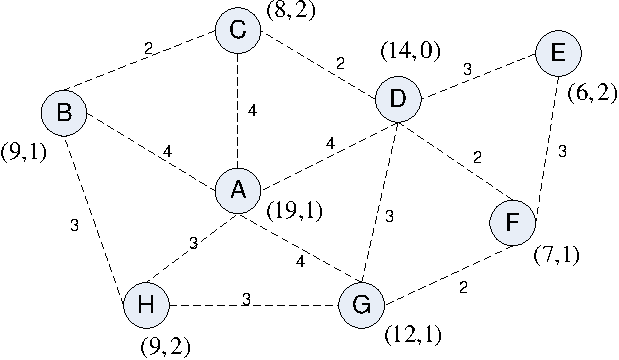
\includegraphics[width=0.7\linewidth]{figure1.pdf}
% 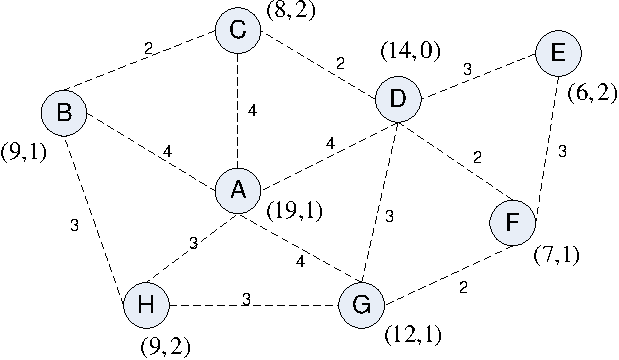
\includegraphics{figure1.pdf}
	\caption{Connectivity graph and the connectivity vector $\{D_i, G_i\}$ on each node. The available channels sensed by each CR node are: $V_A=\{1,2,3,4,5,6,10\}, V_B=\{1,2,3,5,7\}, V_C=\{1,3,4,10\}, V_D=\{1,2,3,5\}, V_E=\{2,3,5,7\}, V_F=\{2,4,5,6,7\}, V_G=\{1,2,3,4,8\}, V_H=\{1,2,5,8\}$. Dashed lines indicates two end nodes are within transmission range of each other. Each edge is labelled by the number of common channels between the two ends.}
	\label{fig1}
\end{figure}

After introducing connectivity vector, we proceed to introduce the first phase of algorithm ROSS.
At first, cluster heads are determined, then clusters are formed on the basis of the cluster heads' neighbourhoods.


\subsubsection{Determining Cluster Heads and Form the Initial Clusters}
In this phase, each CR node decides whether it is cluster head by comparing its connectivity vector with its neighbours.
When CR node $i$ has bigger individual connectivity degree than any neighbours except for those which have already become cluster heads (the appearance of cluster heads will be explained in next subsubsection), then node $i$ becomes clusters head.
%In other words, CR node $i$ becomes cluster head if $D_i > D_k, \forall k\in \texttt{Nb}_i\setminus CHs$ ($CHs$ donate the cluster heads existing in $\texttt{Nb}_i$).
If there is another CR node $j$ in its neighborhood, which has the same individual connectivity degree with $i$, \ie $D_j = D_i$ and $D_j > D_{k}, \forall k\in Nb_j\setminus \{CHs\cup i\}$, then the node out of $\{i, j\}$ with higher social connectivity degree becomes cluster head, and the other one becomes one member of it. 
If $G_i = G_j$ as well, node ID is used to break the tie, \ie the one with smaller node ID takes precedence and becomes cluster head.
%
The node which becomes cluster head broadcasts a message on its eligibility of being cluster head to notify its neighbours, and claims its neighbourhood as its cluster.
The pseudo code for deciding cluster head and forming initial clusters is in Algorithm~\ref{alg0} in appendix.

After receiving the notification from a cluster head, a CR node, \eg $i$, is aware that it becomes one member of a cluster, then $i$ sets its individual connectivity degree to zero. %, which is smaller than all the possible individual connectivity degrees in the CR network.
Then node $i$ broadcasts its new individual connectivity degree to all its neighbours. 
%wrong:
%Note that there is no cluster head which receives the notification on cluster head eligibility, and there is a Lemma on this.
%\begin{theorem}{lemma}
%There is no cluster head receiving the notification message on cluster head eligibility, which is sent from a node which newly becomes a cluster head.
%\end{theorem}
%\begin{proof}
%We use contradiction to prove. 
%Assume a CR node $j$ is cluster head, and receives a notification on cluster head eligibility form CR node $i$. 
%According to the assumption on the reciprocal communication link, $i$ should have received the notification message from $j$ when $j$ becomes cluster head.
%Then CR node $i$ will set its individual connectivity degree to zero, and has no possibility to become a cluster head.
%\end{proof}
When a CR node $i$ is associated to multiple clusters \ie $i$ receives multiple notifications on cluster head eligibility from different CR nodes, $D_i$ is still set to zero. %Note here that connectivity degree on cluster head will still be the actual value.% The value will expire after some duration and is changed later on back to the original value. 
%
%
The purpose of this temporary manipulation on individual connectivity degree is to let the CR nodes out side of the cluster be possible to become cluster heads, so that every CR node either becomes cluster head or a member of at least one cluster.
%In other words, with this manipulation on its individual connectivity degree, every CR node in the network will be involved in the clustering process, the proof will be given later.
%Every CR user is involved in the clustering process and becomes either cluster head or member is described in theorem~\ref{clustering:theorem}.
We have the following theorem to show that as long as a secondary user's connectivity the CRN is not zero, the secondary user will always be integrated into a certain cluster.
\begin{theorem}
\label{clustering:theorem}
Given a CRN, every secondary user is included into at least one cluster within $N$ steps.
\end{theorem}
The Proof is in Appendix~\ref{proof_clustering:theorem}.
According to Theorem~\ref{clustering:theorem}, we can assign reasonable amount of time for phase I to complete.

%This judgement is conducted periodically, and phase I ends after every node ascertains it is cluster head or not.
Let us apply Algorithm~\ref{alg0} to the example shown in Figure~\ref{fig1}.
Node $B$ and $H$ have same individual connectivity degree, $D_B=D_H$, but as $G_H=2>G_B=1$, node $H$ becomes cluster head.
Cluster $C_H$ is $\{H, B, A, G\}$.
	




\subsubsection{Guarantee Availability of Common Control Channel}
After deciding itself being cluster head, CR node broadcasts to notify its neighbours on the dedicated control channel, meanwhile, $i$'s initial cluster is formed immediately, which is $i$'s neighborhood except for those nodes which have become cluster heads, \ie $C_i=(\texttt{Nb}_i\setminus CHs)\cup i$.
Note this is the initial cluster, as it is possible for the formed cluster to pose no common control channels.
This problem can be solved with the following method.

As smaller cluster size increases the number of CCCs within the cluster, certain nodes are eliminated until there is at least one common control channel.
The elimination of nodes is performed according to an ascending list of nodes which are sorted by their number of common channels with the cluster head. 
In other words, the cluster member which has the least number of common channels with the cluster head is excluded first.
If there are nodes having the same number of common channels with cluster head, the node whose elimination brings in more common channels will be excluded.
If this criterion meets a tie, the tie will be broken by deleting the node with smaller ID.
It is possible that the cluster head excludes all its neighbours and resulting into a singleton cluster composed by itself.
%At the end of this procedure every formed cluster has at least one common channel.
The pseudo code for cluster head to obtain at least one common channel is shown in Algorithm~\ref{alg_size_control_available_CCC}.
As to the nodes eliminated in this procedure, they restore their original individual connectivity degrees, and become either cluster heads or get included into other clusters later on according to Theorem~\ref{clustering:theorem}.




\subsubsection{Cluster Size Control in Dense CRN}
\label{cluster_pruning}

In the introduction section, we have stated that cluster size should be given consideration to justify the concept of robustness of clusters, \ie without specifying requirement on cluster sizes, small clusters will be generated to obtain more CCCs.
Except for cooperative sensing, clusters need to conduct some other functionalities.
When cluster size is large, there will be substantial burden on cluster heads to manage the cluster members, which is a challenge for resource limited cluster heads, thus the cluster size should fall in a desired range~\cite{Chen04clusteringalgorithms, capacity_cluster_06}.
Here we illustrate the pressing necessity to control cluster size when CRN becomes dense via theoretical analysis and simulation.

Assuming the CR and primary users are evenly distributed and primary users occupy the licensed channels randomly, then both CR nodes density and channel availability in the CRN can be seen as homogeneous.
Based on Algorithm~\ref{alg0}, cluster heads are the CR nodes which possess the biggest individual connectivity degrees in their neighborhood respectively, and they are surrounded by CR nodes.
%In contrast, CR nodes residing on edge are unlikely to become cluster heads as their neighbourhoods are only half the nodes locating away from edge.
The formed clusters are the neighborhood of cluster heads, which is decided by the transmission range and network density.

When the CRN is extremely dense, consider a cluster with cluster head of CR node $i$, based on the rule for cluster head selection Algorithm~\ref{alg0}, the nearest cluster head could locate just outside node $i$'s transmission range.
An instance of this situation is shown in Figure~\ref{clusters_denseNetwork}.
%
In the figure, black dots represent cluster heads, the circles denotes the transmission ranges of those cluster heads.
Cluster members are not shown in the figure.
%Circles represent the transmission range of cluster head, within which CR nodes are absorbed in cluster.
\begin{figure}[h!]
  \centering
  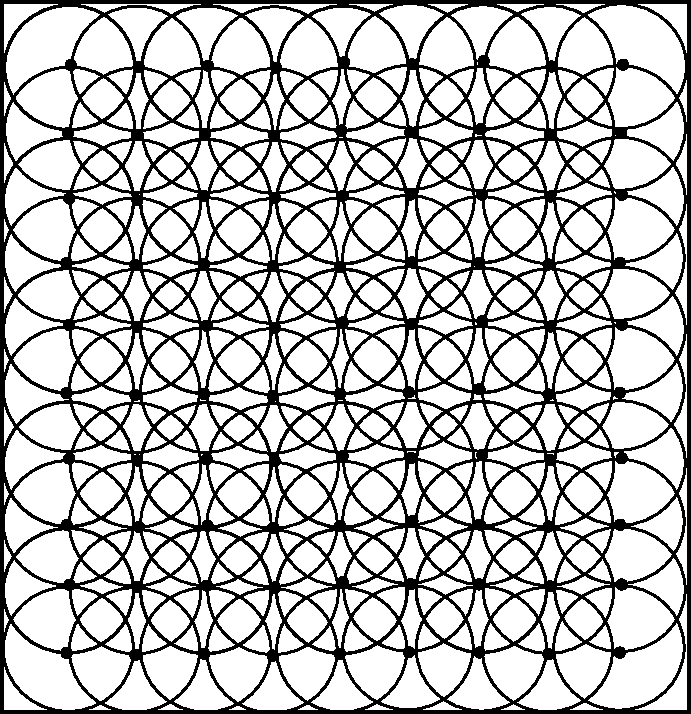
\includegraphics[width=0.4\linewidth]{clusters_denseNetwork_2.pdf}
  \caption{Clusters formation in extremely dense CRN. Black dots are cluster heads, other cluster members are not drawn.}
  \label{clusters_denseNetwork}
\end{figure}
Let $l$ be the length of side of simulation plan square, and $r$ be CR's transmission radius.
Based on the aforementioned analysis and geometry illustration as shown in Figure~\ref{clusters_denseNetwork}, we can give an estimate on the maximum number of generated clusters, which is the product of the number of cluster heads in row and line, $l/r * l/r = l^2/r^2$.

Now we verify the estimation with simulation.
We distribute CR and primary users randomly on a square plain, $r$=10 and $l$=50.
Network density is increased by adding more CR users.
%We now have a look at how does the network density affect the cluster size when the transmission range is constant.
%This implicates when the cluster size is decided by the density of the network.
%As to SOC, the membership of one cluster is decided after a complex process, and the cluster size is roughly the same with one neighborhood.xxxx
%We can see from the example that although two neighbouring clusters can overlap greatly with each other, no cluster head will be covered by other clusters.
The number of formed clusters is shown in Figure~\ref{number_clusters_scale}.
With the increase of CR users in the network, network density increases linearly (the Y axis label is the number of neighbours), and the number of formed clusters also increases and approaches to the the upper bound of 25 which complies with the estimation.
For each network scale, simulation is run for 50 times and the confidence interval is 95\%.

\begin{figure}[h]
  \centering
  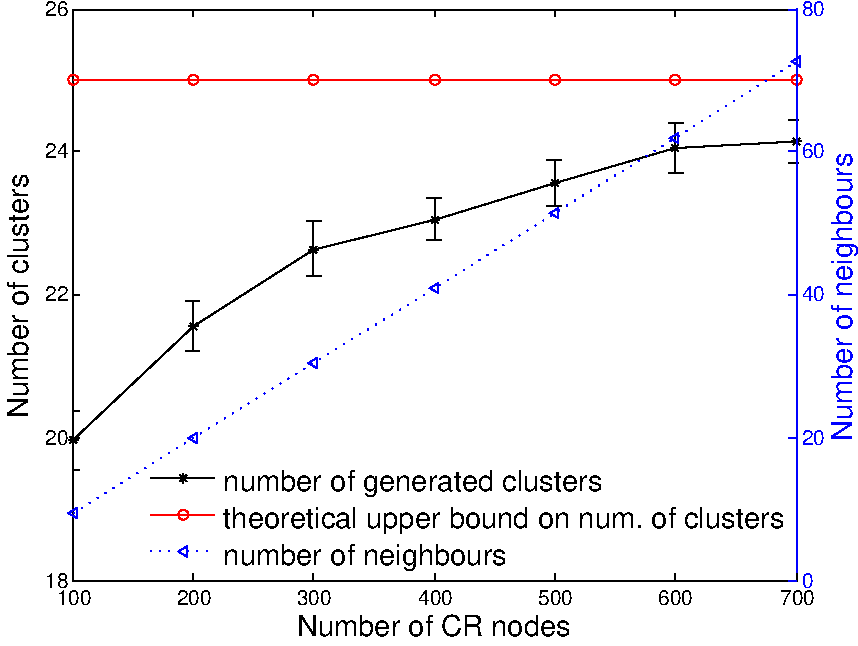
\includegraphics[width=0.8\linewidth]{number_clusters_upperBound.pdf}
  \caption{The correlation between the number of formed clusters and network density. Note that the number of neighbours denotes the network density.}
  \label{number_clusters_scale}
\end{figure}

Both the analysis and simulation show that when applying ROSS, the cluster size increases with the increase of network density.
As a result, certain measures are needed to prevent the network size from increasing with the increasing network density.
This task falls to the cluster heads.
To control cluster size, cluster heads prune their cluster members.
The desired size $\delta$ is decided based on the capability of the CR users and the tasks to be conveyed.
Given desired size as $\delta$, cluster head excludes members sequentially, whose absence leads to the maximum increase of common channels within the cluster.

Note that ROSS generates clusters on based of cluster heads' neighbourhood, thus the $\delta$ is smaller than the average neighbourhood size.
As there are extensive overlaps between clusters, the threshold that the cluster size satisfies requirement should be larger than $\delta$.
%In practise, we set this threshold as $5*\delta/2$.
%This process ends when the size of resultant cluster is at most $5*\delta/2$ and at least one CCC is available.
This process ends when the size of resultant cluster is at most $\delta$ and at least one CCC is available.
This procedure is similar with that to guarantee CCCs in cluster, thus the algorithm can reuse Algorithm~\ref{alg_size_control_available_CCC}.



%Figure~\ref{fig2} shows the clusters formed in the example in Figure~\ref{fig1} when the desired cluster size is 3. 

%Especially, it forster the connectivity between the clusters. It can do so, as the nodes with larger connectivity degree are not cluster heads but members. 
%As basin nodes have smaller $d_i$ compared with its cluster members, and many of the cluster members locate between the basin node and neighbor clusters,  %the bigger $d_i$ with bigger robustness of Social Connection, i.e, with bigger $d$ are located around cluster heads, 
%After clusters are formed, with aid of \textit{control channel rotation scheme} proposed in \cite{Lazos09}, intra and inter cluster communication is conducted and for each debable node (XXX Debatable nodes are not defined yet), the membership and channel availablity of the clusters concluding it is known. 


\begin{figure}[ht!]
  \centering
  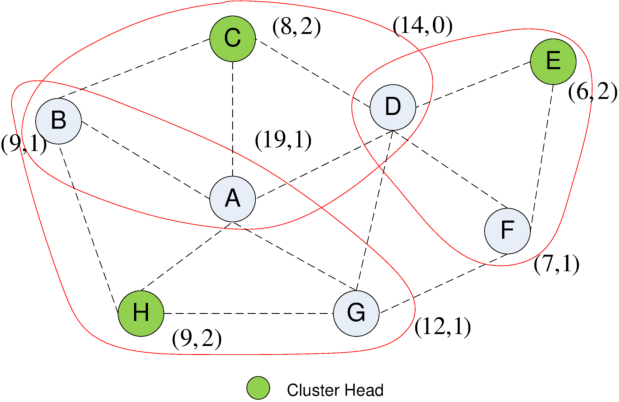
\includegraphics[width=0.6\linewidth]{figure2.pdf}
  \caption{Clusters formation after the first phase of ROSS. There are some nodes being debatable nodes, \ie belonging to more than one cluster.}
  \label{fig2}
\end{figure}


\subsection{Phase II - Membership Clarification}
%\subsubsection*{Problem Description}
After applying phase I of ROSS to the example in Figure~\ref{fig1}, the resulted clusters are shown in Figure~\ref{fig2}.
We notice nodes $A, B, D$ are included in more than one cluster. 
We refer these nodes as \textit{debatable nodes} as their cluster affiliations are not clear, and the clusters which include debatable node $i$ are called \textit{claiming clusters} of node $i$, and are represented as $S_i$.  
Actually, debatable nodes extensively exist in CRN with larger scale.
Figure~\ref{percentage_overlapping_node} shows the percentage of debatable nodes increases when the CRN network scales up.

Debatable nodes should be exclusively associated with only one cluster and removed from the other claiming clusters, this procedure is called cluster membership clarification.
We will introduce the solution for cluster membership clarification in the following.

\begin{figure}[ht!]
  \centering
  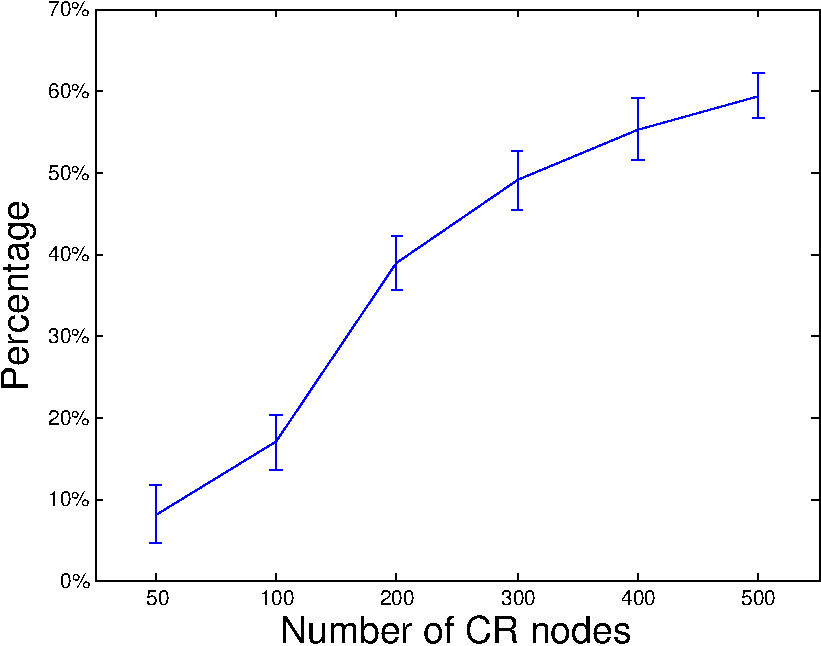
\includegraphics[width=0.7\linewidth]{percentage_overlapping_node.pdf}
  \caption{The percentage of debatable nodes after phase I of ROSS.}\label{percentage_overlapping_node}
\end{figure}



%In the second phase of ROSS, debatable nodes will chose only one cluster to reside.

%In particular, the un-affiliation of one debatable nodes from a cluster increasing the set $K_C$ of ICCs of cluster $C$ (at the cost of potentially decreasing $R_C$, the set of OCCs).

%\newtheorem{observation}{Observation}
%\label{observation}
%\begin{observation}
%If the number of nodes within a cluster decreases, the number of common channels will increase or keep constant.
%\end{observation}
%
%\begin{proof}
%Contradiction, To be continued
%\end{proof}
%From observation 1 we know that the procedure of membership clarification will increase the set of common channels for some clusters and accordingly strengthen the robustness of intra connectivity. 

% % % % %	dependancy!
%An debatable node belongs to multiple clusters, and in the same time, it is possible that several debatable CR nodes locate within one same cluster. %Each debatable node tries to increase the sum of ICC of the clusters which it belong to. More specifically, 
%For a debatable node $i\in S_i$ after phase I, as to clarify its membership, it will choose one cluster $C\in S_i$ to stay and withdraw from the other clusters in $S_i$ with the consideration of increasing ICCs within $S_i$ by the largest margin. 

\subsubsection{Distributed Greedy Algorithm}
%Debatable node $i$ is aware of all its claiming clusters in $S_i$. 
After Phase I, debatable nodes, \eg $i$ needs to decide which cluster $C\in S_i$ to stay, and thereafter leaves the rest others in $S_i$.
The principle for debatable node $i$ to choose one claiming cluster is to result in the greatest increase of common channels in all its claiming clusters.
%The set of available channels of one cluster are known by the debatable nodes which locate in that cluster. %this is finished 
Node $i$ communicates with all the cluster heads whose clusters of its claiming clusters, and is aware of the vector of common channels of the claiming clusters, then $i$ is able to know how many more common control channels will be in one certain claiming cluster if $i$ leaves that cluster.
Based on this calculation, $i$ decides on one claiming cluster to stay and leaves the other claiming clusters.
If there exists one cluster $C\in S_i$, if $i$ leaves this cluster brings the least increased common control channels than leaving any other claiming clusters, then $i$ chooses to stay in cluster $C$.
When there comes a tie in terms of the increase of common channels among multiple claiming clusters, $i$ chooses to stay in the cluster whose cluster head shares more common channels with $i$.
In case there are multiple claiming clusters demonstrating the same on the aforementioned metrics, node $i$ chooses to stay in the claiming cluster with smallest size.
IDs of cluster heads will be used to break tie if the previous rule could not decide on the unique cluster to stay.

Algorithm for debatable node $i$ to decide which claiming cluster to stay is described as Algorithm~\ref{alg4}.
To conduct Algorithm~\ref{alg4}, debatable node $i$ needs to know the necessary information about its claiming clusters, \ie $V_C$ (the set of available channels in $C$), $V_{H_C}$ (the set of available channels on $C$'s cluster head $H_C$) and $|C|, C\in S_i$ (sizes of $i$'s claiming clusters).
After deciding which cluster to stay based on Algorithm~\ref{alg4}, node $i$ notifies all its claiming clusters, and retrieves the updated information of the necessary information $V_C$, $V_{H_C}$, $|C|$, where $C\in S_i$.



This procedure raises the concern on the infinite chain effect that debatable nodes update their choices based on other debatable nodes' choices, and this process never ceases.
Consider the following example, where debatable node $i$ locates in cluster $C\in S_i$, and $C$ has more than one debatable node except for $i$.
Assuming that $i$ makes decision on which cluster to stay, which is followed by the other debatable nodes $j$ to decides its affiliation, and there is $j\in C\in S_i$.
The choice of $j$ may change $C$'s members, \ie $j$ leaves cluster $C$, which could possibly triggers node $i$ to alter its previous decision.
%To maximize the increase of common channel in clusters in $S_j$, $j$ either stays in $C$, or leaves cluster $C$ and stay another cluster in $S_j$.
%$j$'s decision changes $C$'s membership, which will affect $i$'s decision.
%Assume $i$ makes decision before $j$ and chooses to stay in $C$, as which brings the most common channels in $i$' claiming clusters, and then it is $j$' turn to choose cluster.
%If $j$ leaves $C$, the smaller cluster $C$ will possibly make $i$ to leave it and join another cluster.
%and the choice of $j$ to stay in $C$ or not possibly changes $C$'s membership and  which potentially further triggers node $i$ to alter its previous decision. 
Thence, we must answer this question raised when implementing ROSS-DGA.
%, and if it converges, how good such a distributed scheme performs. 
In the following we show that the process of membership clarification can be formulated into a singleton congestion game, and a equilibrium is reached after a finite number of best response updates.

\subsubsection{Bridging ROSS-DGA with Congestion Game}
\label{clustering:phaseII:game}
%In this part, we illustrate that when debatable nodes decide on the exclusive clusters to stay, in particular, the 
To formulate the problem of membership clarification for the debatable nodes in the context of a game, we observe this process from a different (or opposite) perspective. 
From the new perspective, the debatable nodes are regarded as isolated and don't belong to any cluster, which means their claiming clusters become their neighbouring clusters. 
Then for debatable nodes, the previous problem of deciding which clusters to leave becomes a new problem that which cluster to join.
In this new problem, debatable node $i$ (note now $i\notin S_i$) chooses one cluster $C$ out of $S_i$ to join if the decrement of common channels in cluster $C$ is the smallest in $S_i$, and the decrement of CCCs in cluster $C$ is $\sum_{C\in S_i}\Delta\vert K_C \vert=\sum_{C\in S_i}({\vert K_{C} \vert-\vert K_{C\cup i} \vert})$.
The relation between debatable nodes and claiming clusters is shown in Figure~\ref{debatable_nodes_claiming_cluster}.
The concern on convergence appears again as we have discussed in the previous subsubsection.
We will give proof on convergence under game theoretic framework.
\begin{figure}[ht!]
  \centering
  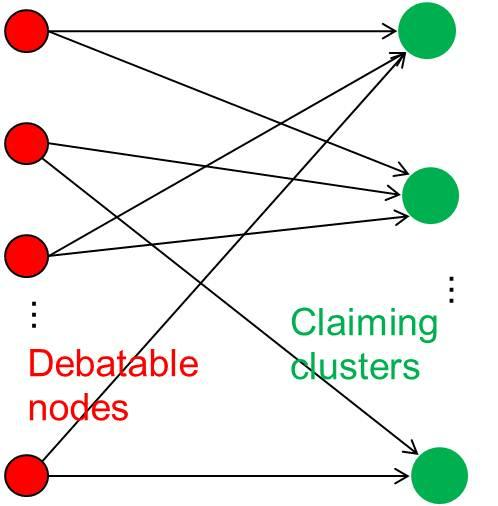
\includegraphics[width=0.25\linewidth]{singletongame_png.png}
  \caption{Debatable nodes and claiming clusters}
  \label{debatable_nodes_claiming_cluster}
\end{figure}

Game theory is a powerful mathematical tool for studying, modelling and analysing the interactions among individuals.
A game consists of three elements: a set of players, a selfish utility for each player, and a set of feasible strategy space for each player. In a game, the players are rational and intelligent decision makers, which are related with one explicit formalized incentive expression (the utility or cost).
Game theory provides standard procedures to study its equilibriums~\cite{game_for_communication_01}.
In the past few years, game theory has been extensively applied to problems in communication and networking~\cite{Neel06analysisand, Wang_gtc_crn_survey_2010}.
Congestion game is an attractive game model which describes the problem where participants compete for limited resources in a non-cooperative manner, it has good property that Nash equilibrium can be achieved after finite steps of best response dynamic, \ie each player choose strategy to maximizes/minimizes its utility/cost with respect to the other players' strategies.
Congestion game has been used to model certain problems in internet-centric applications or cloud computing, where self-interested clients compete for the centralized resources and meanwhile interact with each other.
For example, server selection is involved in distributed computing platforms~\cite{Cloud_Computing_2010}, or users downloading files from cloud, etc.
In the following we will introduce an \textit{server matching}~\cite{kothari:congestion_serverMatching} problem to illustrate congestion game's application in communication systems.


In the following, we show that the decision of debatable nodes to clarify their membership can be mapped to the behaviour of the players in a \textit{player-specific singleton congestion game} when proper cost function is given.

The game to be constructed can be represented by a 4-tuple $\Gamma=(\mathcal{P},\mathcal{R},(\sum_i)_{i \in \mathcal{N}},\Delta\vert K^i_C \vert)$, where the elements in $\Gamma$ are given below,
%To make the model of this game more clear, we make some change to our original problem. Previously, the nodes in overlapping areas belong to more than one cluster, and our scheme is to remove them out of some clusters to increase the set of common channels within the cluster form which the mode leave. In the new model, we assume all the nodes in overlapping nodes don't belong any cluster and the problem become into how do these nodes decide which cluster to join.

%The components of the game are listed as follows,

\begin{itemize}
%	\item $\mathcal{D}=\left\{1,\ldots,n\right\}$, the set of players (debatable nodes).
	\item $\mathcal{P}$, the set of players of the game, which are the debatable nodes after phase I in our clustering problem.
%	\item $\mathcal{R}=\left\{1,\ldots,m\right\}$, the set of resources which player can choose, which are all the clusters in our model.
	\item $\mathcal{R} = \cup S_i, i\in \mathcal{P}$, denotes the set of resources for players to choose, $S_i$ is the set of claiming clusters of node $i$. $\mathcal{R}$ is the set of claiming clusters after phase I in our clustering problem.
	\item As to the strategy space $\sum_i$ of player $i\in \mathcal{N}$, there is $\sum_i \subseteq 2^{\left[S_i\right]}$. As one debatable node is supposed to choose one claiming cluster in our problem, thus only one resource is allocated for $i$, accordingly this congestion game is a singleton game.
	%when $i$ makes decision, only one resource (one claiming cluster) from the allowed resources is allocated.
	
	%\item We denote by $\mathcal{S}=\left(\mathcal{S}_1,\ldots,\mathcal{S}_n\right)\in \sum_1\times \cdots\times\sum_n$ the state of game where player $i$ plays strategy $\mathcal{S}_i\in \Sigma_i$.
	
	\item %For the clusters which are possible destination of debatable nodes, the decrement of common channels caused by different debatable node' join can be different because of the heterogeneity of channel availability within itself and on the debatable nodes. %furthermore, the sequence of debatable node's join can also alter the decrement. 
	The utility (cost) function $f(C)$ of resource $C\in \mathcal{R}$, (or to say $f(r)$ of resource $r \in \mathcal{R}$) is $\Delta\vert K^i_C \vert$ which represents the decrement of CCCs in cluster $C$ caused by debatable node $i$' joining in it.
	As to cluster $C\in S_i$, the decrement of CCCs caused by the enrolment of debatable nodes is $\sum_{i:C\in S_i, i\rightarrow C} \Delta\vert K^i_C \vert$. 
$i\rightarrow C$ means $i$ joins in cluster $C$.
Obviously this function is non-decreasing with respect to the number of nodes joining in cluster $C$.
	
The utility function is not purely decided by the number of players (debatable nodes) as that in a canonical congestion game, because in this game the channel availability on debatable nodes is different.
Given two same sized groups of debatable nodes, when the nodes are not completely the same (neither are the channel availabilities on these nodes), the cost happened on one claiming cluster could be different if the two groups of debatable nodes join in that cluster respectively.
%In a canonical congestion game, the cost (or pay off) is function of only the number of players occupying the resource, and is mono-
%In this new game, the cost function 
Hence, this game is called player specific.
In this game, every player greedily updates its strategy (choosing one claiming cluster to join) if joining in a different claiming cluster minimizes the decrement of CCCs $\sum_{i:C\in S_i} \Delta\vert K^i_C \vert$, player's strategy in the game is exactly the same with the behaviour of debatable node in membership clarification phase, as described by Algorithm~\ref{alg4}.


%	\item The Rosenthal's potential function \cite{Rosenthal} of this congestion game is given by:
%	\begin{equation*}
%	\phi(S)=\sum_{C\in\mathcal{R}} \sum_{i:C\in S_i} \Delta\vert K^i_C \vert   	
%   	%\sum_{i=1}^N \Delta^{i}_{p}(S)=\sum_{i=1}^N \sum_{r\in S_i}\Delta^{i}_{r}(t)	
%  	% \Delta =\sum_{i=1}^N w_i (x_i - \bar{x})^2 .
%	\end{equation*}
%All the players in this game greedily update their strategy to minimize the potential function (congestion), this process is exactly the same with the network behaviour under \textit{Distributed Greedy Algorithm}. 

%	\item It is an asymmetric game because the sets of strategies shared by different players are different.
%	\item The total cost is: 
%\begin{equation*}
%   \sum_{i=1}^N \Delta^{i}_{p}(S)=\sum_{i=1}^N \sum_{p\in s_i} \Delta^{i}_{p}(n_p(S))
%  % \Delta =\sum_{i=1}^N w_i (x_i - \bar{x})^2 .
%\end{equation*}

%This is the global objective we want to minimize.
\end{itemize}

%Singleton congestion game is a special type of matroid game~\cite{Milchtaich1996111,}. 
%It is known that player-specific matroid congestion game admit pure equilibrium, 

As to singleton congestion game, there exists pure equilibria which can be reached with best response update, and the upper bound of number of steps before convergence is $n^2*m$~\cite{Ackermann06purenash}, where $n$ is the number of players, and $m$ is the number of resources.
In our problem, the players are the debatable nodes, and the resources are the claiming clusters (or clusters heads).
Thus the upper bound of the number of steps can be expressed as $\mathcal{O}(N^3)$.
In fact, the actual number of steps is much smaller than $N^3$ as both $n$ and $m$ are considerably smaller than $N$.
The amount of debatable nodes is illustrated in Figure~\ref{fig2}, which is between 10\% to 80\% of the total number of CR nodes in the network.
The number of clusters heads, as discussed in the part of cluster size in Section~\ref{phaseI}, is decided by the network density and the CR node's transmission range.
Only a small part of the CR nodes become cluster heads, as in the example shown in Figure~\ref{number_clusters_scale}, the number of clusters is only 3.4\% to 20\% of the total number of CR nodes.



%and the number of steps towards \textit{Nash Equilibrium} is upper-bounded\footnote{Here we present this with modifying the original conclusion in \cite{Ackermann06purenash} according to our model.} by $ n^2\cdot m $. In our context, $n$ is the number of debatable nodes, $m$ is number of clusters in CRN, %$rk(\Gamma)$ of the matroid  is the cardinality of the maximal independent sets, which is 1 in the case of singleton game, 
%so the total time complexity to achieve the \textit{Nash Equilibrium} using greedy approach is 	.
%%(XXX Just mention after this complexity result the relationship to the system mdeol XX)
%This is upper-bounded (in the worst case) by $O(\vert I\vert^3)$. 
%Based on above model and analysis, phase II converges is Algorithm~\ref{alg4} is run by debatable nodes. 
%Although the game version of DGA can achieve \textit{Nash Equilibrium}, the whole scheme can possibly obtain sub-optimal result.    %, furthermore,this stable state is a local minimum of the global decrement function.
%\todo[inline]{The number of steps, or the upper bound of steps in convergence needs a formal proof}

\subsubsection{Distributed Fast Algorithm (DFA)}
%The convergence speed of DGA is large recalling that the number of steps is of $\mathcal{O}(N^3)$.
We propose a faster version of ROSS, which is ROSS-DFA, which is especially suitable for CRN where channel availability change dynamically and re-clustering is necessary.
In DFA, debatable nodes regard their claiming clusters includes all their debatable nodes, thus the membership of claiming clusters is static and debatable nodes can make decisions simultaneously without considering the change of membership of their claiming clusters.
To run ROSS-DFA, debatable node executes only one loop in Algorithm~\ref{alg4}.

Now we apply the two versions of ROSS to the toy network in Figure \ref{fig2}, which has finished cluster head selection.
In the network, node $A$'s claiming clusters are cluster $C_C, C_H\in S_A$, their members are $\{A,B,C,D\}$ and $\{A,B,H,G\}$ respectively. 
The two possible strategies of node $A$'s clarification is illustrated in Figure \ref{fig3}.
In Figure \ref{AinC}, node $A$ staying in $C_C$ and leaving $C_H$ brings 2 more CCC into $S_A$, which is more than that brought by another strategy showed in \ref{AinH}.
After the decisions made similarly by the other debatable nodes $B$ and $D$, the final clusters formed are shown in Figure~\ref{fig4}.

%Using DFA in phase II, the time complexity is decreased drastically to 1. Thus, the total complexity of ROSS-DFA is $|I|$, while, ROSS-DGA's complexity is $|I|^3$ in the worst case.


\begin{figure}[h]
\centering
\subfigure[Node A stays in cluster $C_C$, quits $C_H$, $\Delta\vert K_{C_C}\vert+\Delta\vert K_{C_H}\vert=2$]{
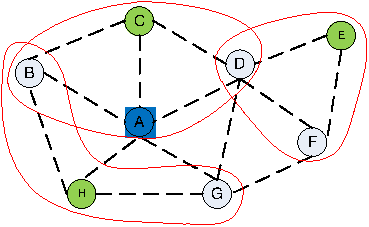
\includegraphics[width=0.435\linewidth]{figure4AinC.pdf}
\label{AinC}
}
\hspace{.15 in}
\subfigure[Node A stays in cluster $C_H$, quits $C_C$, $\Delta\vert K_{C_C}\vert+\Delta\vert K_{C_H}\vert=1$]{
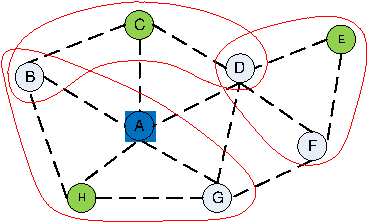
\includegraphics[width=0.435\linewidth]{figure4AinH.pdf}
\label{AinH}
}
\caption[]{Membership clarification: possible cluster formations decided by node A's different choices} %\subref{node A in $C_C$}, \subref{node A in $C_H$}}
\label{fig3}
\end{figure}

\begin{comment}
As an example, when node A comes to decide which cluster to stay, the memberships of relevant clusters, like $C_C$ and $C_H$, are $\{C,B,D,A\}$ and $\{H,B,G,A\}$ respectively. Before the other two debatable nodes B and D making their belonging clear, cluster $C_C$ and $C_H$ have them in the same time. So node A can decide which cluster to belong to without considering other debatable nodes' action. There are two strategies for node A, which is illustrated in Figure \ref{fig3}. Because staying in cluster $C_C$ brings in more common channels within relevant clusters, node A finally choose cluster $C_C$ to stay and caveat from cluster $C_H$. The membership of $C_H$ is updated in the same time. Node B and D undertake the same process and the clusters are formed finally as Figure \ref{fig4} shows.

Because debatable nodes can conduct membership clarification abased on static membership information of relevant clusters, thus no iteration happens in this process. The time complexity of this algorithm is only decided by the number of debatable nodes, which is maximal $O(\vert I\vert)$. 

As an example, when node A comes to decide which cluster to stay, the memberships of relevant clusters, like $C_C$ and $C_H$, are $\{C,B,D,A\}$ and $\{H,B,G,A\}$ respectively. Before the other two debatable nodes B and D making their belonging clear, cluster $C_C$ and $C_H$ have them in the same time. So node A can decide which cluster to belong to without considering other debatable nodes' action. Figure \ref{AinC}. Because staying in cluster $C_C$ brings in more common channels within relevant clusters, node A finally choose cluster $C_C$ to stay and retreat from cluster $C_H$. The membership of $C_H$ is updated in the same time. Node B and D undertake the same process and the clusters are formed finally as Figure \ref{fig4} shows.
\end{comment}


\begin{figure}[h]
  \centering
  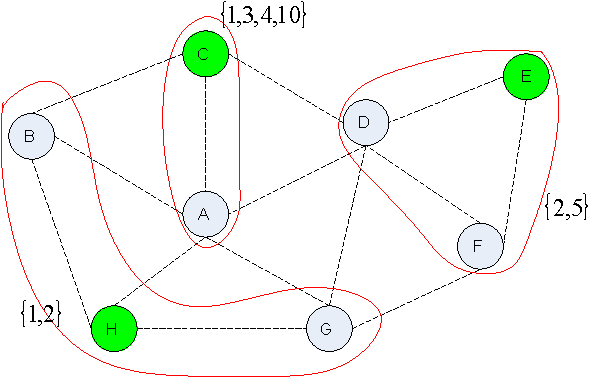
\includegraphics[width=0.5\linewidth]{final_clustering_ross.pdf}
  \caption{Final formation of clusters, CCCs for each cluster is shown.}
  \label{fig4}
\end{figure}



\section{Centralized Clustering Scheme}
\label{centralized_scheme}

%paper given by james is useful which provides a survey from the perspective of wsn!


%\todo[inline]{check}
The centralized clustering scheme aims to form clusters with desired sizes, meanwhile the total number of common control channels of all clusters is maximized.
In the following, we refer this problem as \textit{centralized clustering}, and the problem definition is as follows, 


\begin{mydef}
\label{def_centralized_clustering}
\textit{Centralized clustering in CRN.}

Given a cognitive radio network $\mathcal{N}$ where nodes are indexed from 1 to $N$ sequentially.
Based on certain correlation, certain secondary users constitute one cluster $C$.
$1\leq |C| \leqslant k$ where $|C|$ is the size of cluster $C$ and $k$ is a positive integer.
We name the collection of such clusters as $\mathcal{S}=\{C_1, C_2,\ldots,C_{|\mathcal{S}|}\}$ (the subscript $i$ is the unique index of cluster in $\mathcal{S}$, not the ID of cluster head of that cluster), $\mathcal{S}$ satisfies the following properties: $\bigcup_{1\leq i \leq |\mathcal{S}|} C_i = N$ and $V_{C_i}\neq \emptyset$ for any $i$ which satisfies $1\leq i \leq |\mathcal{S}|$.

Following condition distinguishes the centralized clustering problem discussed in this paper.
The number of common control channels is $|V_{C}|$ if $|V_{C}|>1$, and is zero when $|V_{C}|=1$.
We use $f$ to denoted this new number of CCCs. 
The question of this problem is to find a subcollection $\mathcal{S}' \subseteq \mathcal{S}$, so that $\bigcup_{C_j\in \mathcal{S}'} C_j = N$, and $C_j'\cap C_j =\emptyset$ for $C_j', C_j\in \mathcal{S}'$, so that $\sum_{C\in \mathcal{S}'} f$ is maximized.
% when $|C|>1$, and $f(\cdot)=0$ when $|C|=1$.
%As to $f(\cdot):z\rightarrow z$, under this problem setting, if only number of common channels are given consideration, only singleton clusters will be preferred, which contradicts to our goal of clustering CR nodes together, thus we choose $f(\cdot)= |V_{C}|\cdot |C|$, the product of number of common channels and cluster size.
The decision version of centralized clustering in CRN is to ask whether exist $\mathcal{S}'\subseteq \mathcal{S}$, so that $\sum_{C\in \mathcal{S}'} f \geqslant \lambda$ where $\lambda$ is a real number.% in stead of to maximize $\sum_{C\in \mathcal{S}'} f$.
\end{mydef}


%The decision version of \textit{weighted exact cover problem}: 
%Given an universe $U$, and collection $S=\{s_1, s_2, \ldots, s_m\}$ where each subset $s_i\subseteq U$ and is given a weight $w_i$, whether there exists a collection of subsets $\mathcal{C}$ and constant number $\lambda$, so that the union of $\mathcal{C}$ equals to $U$, $s_j\cap s_{j'} = \emptyset$ for different $j$ and $j'\in \{1,2,\ldots, m\}$, and $\sum_{i\in J} w_i \geq \lambda$.
\subsection{Complexity of Clustering Problem}
In the following part of this section, we will discuss the complexity of centralized clustering problem and provide a centralized solution for it.

\begin{theorem}
\label{theorem1}
CRN clustering problem is NP-hard, when the maximum size of clusters $k\geqslant 3$.
%Assume a CRN can be represented by a connected graph, and there is at least one common channel between any pair of neighbours, then forming at least two CR nodes into one cluster is NP-complete.
\end{theorem}
The proof is in Appendix~\ref{proof_theorem1}.



\subsection{Centralized Optimization}
\label{centralized_opt}
%Exact cover problem can be solved with Knuth's Algorithm X~\cite{dancingLinks_Knuth} as it finds out all the instances of exact cover, then we can choose the one with the biggest sum of weights. 
As there is no efficient algorithm to solve clustering problem in CRN, we propose a centralized optimization where the objective function and the constraints are heuristic, then we adopt binary linear programming to solve the problem.
%Note that binary linear programming is in NP-complete.

%This example indicates the chose of $\mathcal{C}$ plays an important role on the resultant clustering strategy.
%Meanwhile, it provide a chance to constrain the cluster size by putting groups with desired sizes into $\mathcal{C}$.

%the maximum size of $S$ is the \textit{Bell number} of $N$, and $S$ contains the conditions cluster .
%In this case, the resultant $\mathcal{C}$ is composed with all the singleton clusters, \ie, the cluster which contains one node, and the objective is -38.

%it is possible that there doesn't exist combination of clusters with the same cluster size.
%We thus list all possible clusters whose sizes are from 2 to one certain number \footnote{this number of decided by the density of CR network, along with the occupation of PUs. We set this number as cluster size of the biggest cluster ever appears when conducting distributed schemes.}, and check each combination of clusters to find the best covering of network on the aspect of number of ICCs per cluster.
%The complexity of computation is thus \bigO$(N^\delta)$, $\delta$ is the preferred cluster size.

%The global optimal clustering scheme with respect to the number of common channels is investigated to show the gap with the distributed schemes.


%We apply this centralized scheme on a network with network size $N$ and cluster size $\delta$.
%There is $N\mod \delta=0$, and the expected number of clusters is $C = N/\delta$.
%These tailored parameters don't harm the validity of the performance gap between the two schemes.

Given a CRN $\mathcal{N}$ and desired cluster size $\delta$, we obtain a collection of clusters $\mathcal{G}$ which contains all the \textit{legitimate} clusters, and the sizes of these clusters are $1,2,\ldots,\delta$.
Legitimate clusters are the clusters which satisfy the conditions in Section~\ref{def_cluster}. 
Note that the legitimate clusters include the singleton ones, which guarantees the partition of any network is feasible.

With $N=|\mathcal{N}|, G=|\mathcal{G}|$, we construct a constant $G\times N$ matrix $Q_{G\text{x}N}$. 
The element of matrix $Q$ is $q_{ij}$, where the subscript $i$ denotes a legitimate cluster, and $j$ denotes a CR node, which can be seen as the node ID. 
Note that $C_i$ means $i$th cluster in the collection $\mathcal{G}$, doesn't denote the cluster where cluster head is $i$, this notation is only valid in this subsection.
There are $i\in \{1,2,\cdots,G-1, G\}$, and $j\in \{1,2,\cdots,N-1, N\}$.
Element $q_{ij}= k_{C_i}$ if node $j\in C_i$, and $q_{ij}= 0$ if $j\notin C_i$.
In other words, each non-zero element $q_{ij}$ denotes the number of CCCs of the cluster $i$ where node $j$ resides.

\begin{figure}[ht!]
\centering
Q = \bordermatrix{~ 		& 1 	& 2 	& 3 	& \cdots & j & \cdots	& N-1 	& N	\cr
                  1 	& k_{C_1} 	& k_{C_1} 	& 0 	& \cdots & \cdots &\cdots	& 0 	& 0	\cr
                  2 	& k_{C_2} 	& 0 	& k_{C_2} 	& \cdots & \cdots & \cdots 	& 0 	& 0	\cr
				\vdots  	&\vdots & 	 	& 		&  \vdots		& 		& \vdots \cr
				i 	& 0 	& k_{C_i} 	& 0 	& \cdots  & \cdots & \cdots 	& k_{C_i} 	& 0	\cr
				\vdots  	&\vdots & 	 	& 		&  \vdots & \cdots & \cdots 		& 		& \vdots \cr
				\vdots 	& \vdots  	& 0 	& 0 	& \cdots & \cdots & \cdots 	& k_{C_i'} 	& 0	\cr
				G  	& k_{C_G} & \cdots	 	& 		&  \vdots	& \cdots & \cdots& 		& \vdots \cr}	
\caption{An example of Matrix Q, its rows correspond to all legitimate clusters, and columns correspond to the CR nodes in the CRN.}
\label{xx}
\end{figure}

We build a $G\times N$ binary variable matrix $X$, which illustrates the clustering strategy.
The element of matrix $X$ is binary variable $x_{ij}, i=1, \ldots, G, j=1, \ldots, N$.
$x_{ij}=1$ denotes cluster $i$ is one partition in the clustering solution, $x_{ij}=0$ means this partition is not adopted.
%Note that matrix $Q$ contains only constant elements, and matrix $X$ contains only binary variables.
Now, we can formulate the optimization problem as follows,

\begin{equation}
\begin{aligned}
     &\min\limits_{x_{ij}} && \Sigma_{j=1}^N\Sigma_{i=1}^G (-x_{ij}q_{ij} + (1-w_i)*p) \\
     &\text{subject to}   && \Sigma_{i=1}^G x_{ij} = 1, for \forall j=1, \ldots, N \\
   &&& \Sigma_{j=1}^N x_{ij} = |C_i|*(1-w_i), for \forall i=1, \ldots, G \\
   &&& \text{$x_{ij}$ and $w_i$ are binary variables.}\\
   &&& i\in \{1,2, \cdots G\}, \hspace{0.3cm} j\in \{1,2,\cdots N\}
\notag
\end{aligned}
\end{equation}
The objective is the sum of two parts, the first part is the sum of products of cluster size and the corresponding number of CCCs.
We notice that the first part is the metric adopted by the scheme SOC~\cite{Lazos09}.
The second part is the \textit{punishment} for choosing the clusters whose sizes are not $\delta$.
In fact, the second part is particularly designed to eliminates the drawbacks of SOC, \ie a large number of singleton clusters, or a few very large clusters which access affluent unlicensed spectrum.
In practical computation, we minimize the opposite of the sum of the products of cluster size and the corresponding number of CCCs, thus the punishment is positive.

The first constraint restricts each node $j$ to reside in exactly one cluster.
The second constraint regulates that when $i$th legitimate cluster $C_i$ chosen, the number of elements which equal to 1 in the $i$th row is $|C_i|$.

Now we explain how does the mechanism of the punishment in the objective work. 
$w_i$ is an auxiliary binary variable, which denotes whether cluster $C_i$ is chosen by the solution, in particular, 
$$
w_i = \left\{ \begin{array}{rl}
0 &\mbox{if $i$th legitimate cluster $C_i$ is chosen} \\
1 &\mbox{if $i$th legitimate cluster $C_i$ is not chosen} \\
\end{array} \right.
$$
%$w_i=0$ denotes $i$th legitimate cluster $C_i$ is chosen in the solution, and $w_i=1$ means $i$th legitimate cluster is not chosen.
and $p$ is defined as follows,
%$\texttt{cost($\delta$)}$
$$
p = \left\{ \begin{array}{rl}
0 &\mbox{ if $|C_i|=\delta$} \\
\alpha_1 &\mbox{if $|C_i|=\delta-1$} \\
\alpha_2 &\mbox{if $|C_i|=\delta-2$} \\
\dots
\end{array} \right.
$$
where $\alpha_i>0$ and increases when $|C_i|$ diverges from $\delta$.
Because of $w_i$, any chosen cluster brings certain \textit{punishment}.
Function $p$ denotes that when the chosen cluster's size is desired size $\delta$, the punishment is zero.
When the chosen cluster's size diverges from $\delta$, the objective function suffers \textit{loss}.
%
Choice of $\alpha_i$ affects the resultant clusters.



%\begin{figure}[ht!]
%\centering
%\includegraphics[width=0.45\linewidth]{example.JPG}
%\caption{Example of Matrix Q in a 6-node network, cluster size is set as 2}
%\label{xx}
%\end{figure}

%\begin{figure}[ht!]
%  \centering
%  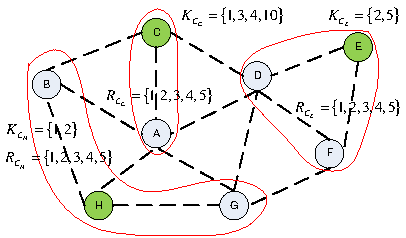
\includegraphics[width=0.5\linewidth]{figure5final.pdf}
%  \caption{Final cluster formation.}
%  \label{fig4}
%\end{figure}



This is a integer linear optimization problem, which is solved by function $bintprog$ provided in MATLAB.
Note that the proposed centralized solution is heuristic.
There are two reasons for pursuing the heuristic scheme, first, the problem of centralized clustering is NP hard, and there is no efficient solution to solve it.
The second reason is, the collection of legitimate clusters is dependant on the network topology and spectrum availability in the network, thus to each specific CRN, the space of solution is different.


\subsubsection{Example of the Centralized Optimization}
We look into how it the centralized scheme perform in the toy example of the CRN in Figure~\ref{fig1}.

We let the cluster size $\delta$ to be 3.
A collection of clusters $\mathcal{G}$ is obtained, which contains all the clusters satisfying the conditions of cluster in Section~\ref{def_cluster} and the sizes of clusters are 1, 2 or 3. 
$\mathcal{G}=\{\{A\}, \{B\},\dots,\{B,C\},\{B,A\},\{B,H\},\cdots,\{B,A,C\},$\\$\{B,H,C\}, \{A,D,C\},\cdots\}$, $G = |\mathcal{G}|=38$.
$\alpha_1$ and $\alpha_1$ are set as 0.2 and 0.8. 
The clustering result of centralized programming is shown in Figure~\ref{fig:final_clustering_LP}.

The formed clusters are $\{\{D,E,F\},\{A,C,G\},\{H,G\}\}$, the numbers of CCCs are 2, 3, 3.
The resulted clustering solutions from ROSS-DGA/DFA and SOC are shown in  Figure~\ref{fig4} and Figure~\ref{fig:final_clustering_soc} respectively.%, clusters are $\{A,B,C,D,G\},\{E,F\},\{H\}$, and the numbers of CCCs are 2, 3, 4.
%The solution resulted from ROSS-DGA is $\{\{B,H,G\},\{C,A\},\{D,E,F\}\}$ (in Figure~\ref{fig4}), the numbers of CCCs are 2, 4, 2.
%ROSS-DFA generates the same result with ROSS-DGA in this example.	
As to the average number of CCCs, the results of ROSS, centralized and SOC are 2.66, 2.66, and 3 respectively. 
Note there is one singleton cluster $C_H$ generated by SOC, which is not preferred.
When the singleton cluster $\{E\}$ is excluded, the average number of common channels of SOC drops to 2.5. 
\begin{figure}[ht]
\begin{center}
\subfigure[Resulted from SOC]{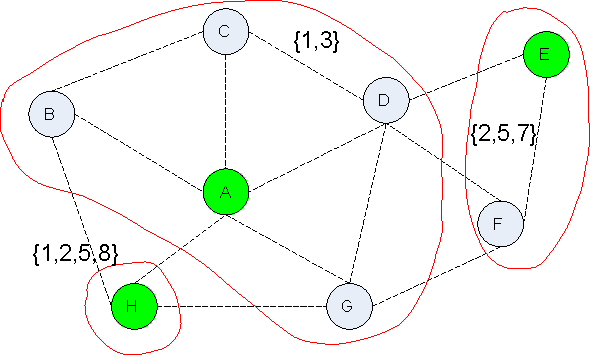
\includegraphics[width=0.435\linewidth]{final_clustering_soc}\label{fig:final_clustering_soc}}
\hspace{0.15 in}
\subfigure[Resulted from Centralized Optimization]{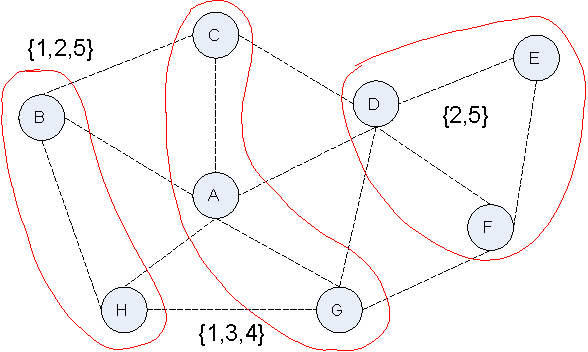
\includegraphics[width=0.435\linewidth]{final_clustering_LP}\label{fig:final_clustering_LP}}
\end{center}
\caption{Final clusters formed in the example CRN network from Figure~\ref{fig1}}
\label{fig:final_clustering}
\end{figure}

 





\section{Performance Evaluation}
\label{performance}
In this section, we evaluate the performances of all the variants of ROSS, \ie ROSS-DGA and ROSS-DFA, and that with cluster size control features.
The latter is referred as ROSS-x-DGA/ROSS-x-DFA, where x is the desired cluster size.
We choose SOC as comparison scheme.
To the best of our knowledge, SOC~\cite{Lazos09} is the only work emphasizing on the robustness of clustering structure from all previous work on clustering in CRN. The authors of~\cite{Lazos09} compared SOC with other schemes based on the average number of common channels within each cluster, on which SOC outperforms other schemes by 50\%-100\%. This is because the schemes except for SOC are designed either for ad hoc network without consideration of channel availability~\cite{Basagni99}, or for CRN  but just considering basic connection among CR nodes~\cite{Zhao07}. Hence, we only compare the two versions of our scheme ROSS-DGA and ROSS-DFA with SOC to show the merits of ROSS, and also compare with the centralized scheme to see the gap with the global optima. 
In particular, we will investigate the following metrics,
\begin{itemize}
\item \textit{Average number of common channels per non-singleton cluster.} 
This metric shows the robustness of the current non-singleton clusters.
Non-singleton cluster refers the cluster whose cluster size is larger than 1, and can also be seen as unclustered node.
Note that this metric along is biased and misleading, because the CR nodes with more channels could be formulated as singleton clusters.
This happens in SOC solution, whose objective is to improve the average number of common channel over \textit{all} clusters, \ie including the singleton clusters, thus many CR nodes with more channels are turned into clusters.
%As we try to look into the robustness of clusters of CRs, we exclude those singleton clusters.


\item \textit{Number of unclustered CRs with moderate and vigorous intensity of primary users' activities.}
This is a straight forward metric which reflects the robustness of clusters, as this metric directly shows how many nodes can make use of the cluster structure.
With this metric, we investigate the performance of different schemes under different availability of spectrum in the CRN.
When we vary the intensity of primary users' activity, \eg from low to medium level by increasing the number of primary users, this metric is the antonym of \textit{survival rate}, \ie, how many nodes are still within a certain cluster when some clusters have collapsed due to the newly added primary users.


\item \textit{Cluster sizes.}
Specific clusters size is pursued in many applications due to energy preservation and the system design ~\cite{clustering_globecom11}.
We will present the distribution of CRs residing in the formed clusters, and the number of generated clusters through multiple simulations.

\item \textit{Amount of control messages involved.}

\end{itemize}

The simulation is conducted with C++. 
Certain number of CRs and PUs are deployed in a 2-dimensional Euclidean space.
We adopt the unit disk model~\cite{unitDiskModel}, and both CR users and PU have fixed transmission ranges respectively.
Complying with the system model, the CR node residing within another CR node's transmission range is seen as neighbour of that CR node.
If CR node locating within one PU's transmission range, the CR node is not allowed to use the channel which is being used by that PU.
The number of licensed channels is 10, each PU is operating on each channel with probability of 50\%.
All primary and CR users are assumed to be static during the process of clustering.

Simulation is divided into two parts, in the first part, we investigate the performance of centralized scheme, and the gap between the distributed schemes with the centralized scheme.
The simulation of this part is conducted in a small network, as there is no polynomial time solution available to solve the centralized problem.
In the second part, we investigate the performance of the proposed distributed schemes thoroughly in the networks with different scales and densities.

\subsection{Centralized Schemes vs. Decentralized Schemes}
10 primary users and 20 CR users are dropped randomly (with uniform distribution) within a square area of size $A^{2}$, where we set the transmission ranges of primary and CR users to $A/3$.
There are 10 available channels. 
With this setting, the average number of neighbours of one CR user is 4.8.
Each primary user randomly occupies one channel, and CR users are assumed to be able to sense the existence of primary users and identify available channels.
When clustering scheme is executed, around 7 channels are available on each CR node.
The desired cluster size is 3, the parameters used in the \textit{punishment} for choosing the clusters with undesired sizes are set as follows, $\alpha_1 =  0.4$, $\alpha_2 =  0.6$.
Performance results are averaged over 50 randomly generated topologies with equal parameters.
The confidence interval shown in figure corresponds to 95\% confidence level.

\subsubsection{Number of Common Control Channels in Non-singleton Clusters}
\label{ccc_20}
%We first have a look at the average number of common channels per non-singleton cluster.
Figure~\ref{ccc_per_nonsingleton} shows the average number of common channel of non-singleton clusters, as the singleton clusters (in other words unclustered nodes) don't execute any functionalities of clusters, which are has be discussed in Section~\ref{intro}.
From Figure~\ref{ccc_per_nonsingleton}, we can see centralized schemes outperform distributed schemes.
SOC achieves the most number of CCC than all the variants of ROSS.
The reason is, SOC is liable to group the neighbouring CRs which share the most abundant spectrum together, no matter how many of them are, thus the number of CCC of the formed clusters is higher.
But this method leaves considerable number of CRs which have less spectrum not in any clusters.
As to the variants of ROSS, the procedure of debatable nodes greedily looking for better affiliation improves the number of CCC, thus ROSS-DGA with and without size control outperform ROSS-DFA and its size control version respectively.
We also notice that, the size control feature doesn't affect the number of CCC for both ROSS-DGA and ROSS-DFA.
This is because the desired cluster size happens to be the average size of clusters generated by ROSS-DGA and ROSS-DFA, then the size control functionality doesn't play effect to increase the number of CCCs.



\subsubsection{Survival Rate of Clusters with Increasing Primary Users}
With the number of PUs in CRN increases, or their operation becomes more intensive, some CCCs will no longer be available.
If there is no common control channels available any more because of the new added PRs, the cluster is regarded as destroyed and the former cluster member CRs become unclustered CRs or in other words singleton clusters.

We investigate the robustness of the formed clusters when they co-exist with primary users whose intensity of activities are varying.
After the clusters are formed under the influence of the initial 10 PUs, extra 100 PUs are added sequentially to the network.
%The transmission range and channel occupancy of the new PU is the same with the previous ones, \ie transmission range is $A/3$, and one channel out of 10 is randomly chosen to operate.
Figure~\ref{singleton_clusters} shows the number of unclustered CRs with the increasing number of PUs.%, which indicates the vulnerability of clusters under varying availability of licensed spectrum.
%
We draw three conclusions corresponding to three comparisons shown in this figure,
\begin{itemize}
\item Centralized scheme with cluster size of 2 generates the most robust clusters, and SOC results in the most vulnerable clusters.
When the desired cluster size is 3, the centralized scheme performs similarly with the variants of ROSS.
The reason that centralized scheme with cluster size of 3 does not completely excel variants of ROSS is due to the favourable achievement of it: the uniformly sized clusters.
As distributed schemes, variants of ROSS generate considerable amount of smaller clusters which are more likely to survive when PUs' activities become intense.
The comparison on cluster sizes will be given in details in~\ref{cluster_size}.
% when the number of PRs is 10$\sim$30, when number of PUs is 30$\sim$60, same amount of unclustered CRs are generated with variants of ROSS.
%When there are 75 and more new PRs, centralized scheme with cluster size of 3 results in more unclustered CR nodes than variants of ROSS.


\item Greedy algorithm improves survival rate. 
ROSS-DGA improves the survival rate of ROSS-DFA, so does ROSS-x-DGA against ROSS-x-DFA.
This complies with the observation in Figure~\ref{ccc_per_nonsingleton}.
As the debatable CRs greedily update their affiliation with claiming clusters, and the metric for updating is the maximum increase of CCCs of the demanding clusters, the average number of CCCs in non-singleton clusters is improved. 
%Meanwhile, sizes of more clusters become smaller also contributes more robustness.

\item ROSS with size control is better than the other two distributed schemes.
Conducting size control improves both ROSS-DGA and ROSS-DFA's performance when the number of new PUs is greater than 50.
The size control decreases the clusters size and makes the clusters more robust when against PUs' activity.

\end{itemize}




%\begin{figure}[h!]
%  \centering
%  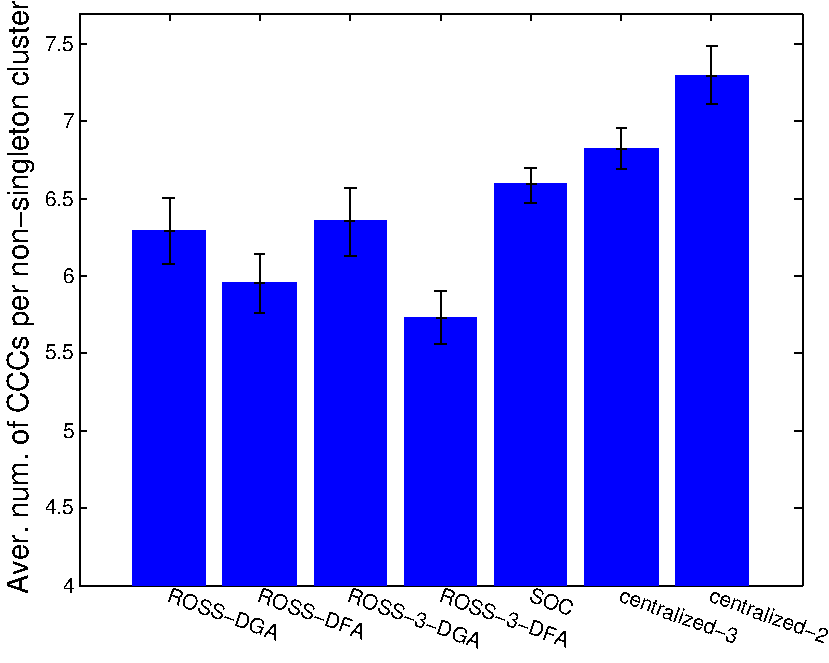
\includegraphics[width=0.8\linewidth]{ccc_20.pdf}
%  \caption{Number of common channels for non-singleton clusters, the numbers in the names of schemes annotate the desired cluster size.}
%  \label{ccc_per_nonsingleton}
%\end{figure}
%
%
%\begin{figure}[h]
%  \centering
%  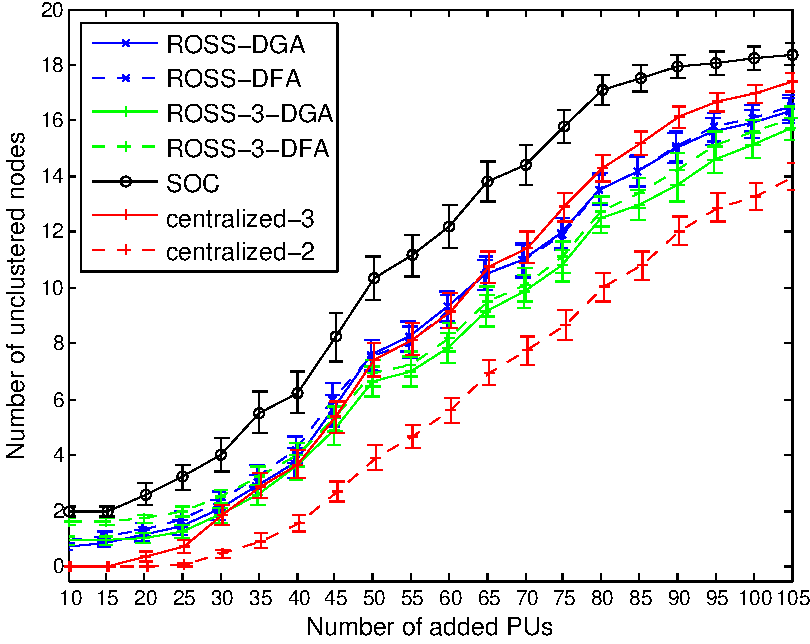
\includegraphics[width=0.8\linewidth]{survival_rate_20.pdf}
%  \caption{Number of CRs which are not included in any clusters}
%  \label{singleton_clusters}
%\end{figure}



\subsubsection{Cluster Size Control}
\label{cluster_size}
%\begin{figure}[h]
%  \centering
%  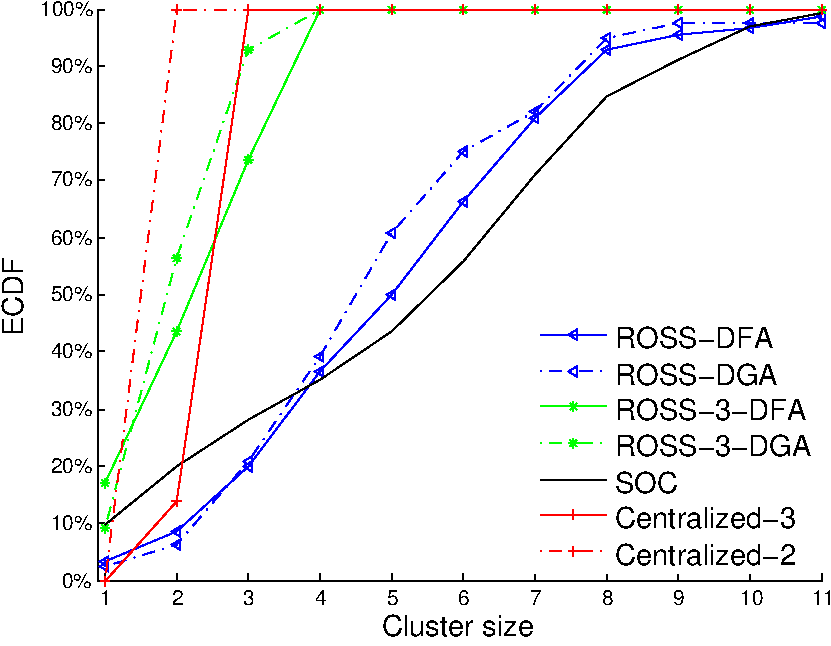
\includegraphics[width=0.8\linewidth]{cdf_clusterSize_20.pdf}
%  \caption{Cumulative distribution of CRs residing in clusters with different sizes.}
%  \label{size_control}
%\end{figure}


\begin{figure*}[t]
\begin{multicols}{3}
    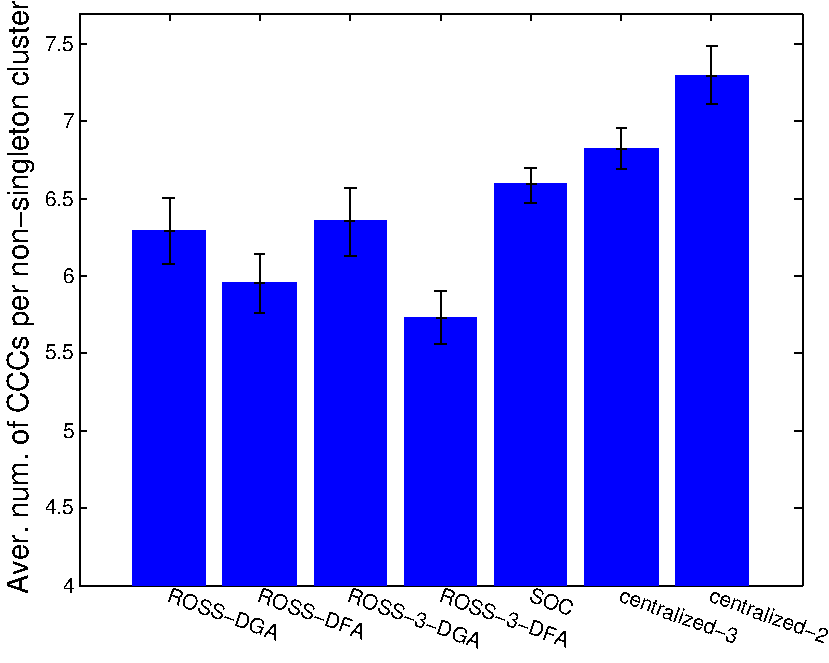
\includegraphics[width=\linewidth]{ccc_20.pdf}\par\caption{Number of common channels for non-singleton clusters}\label{ccc_per_nonsingleton}
    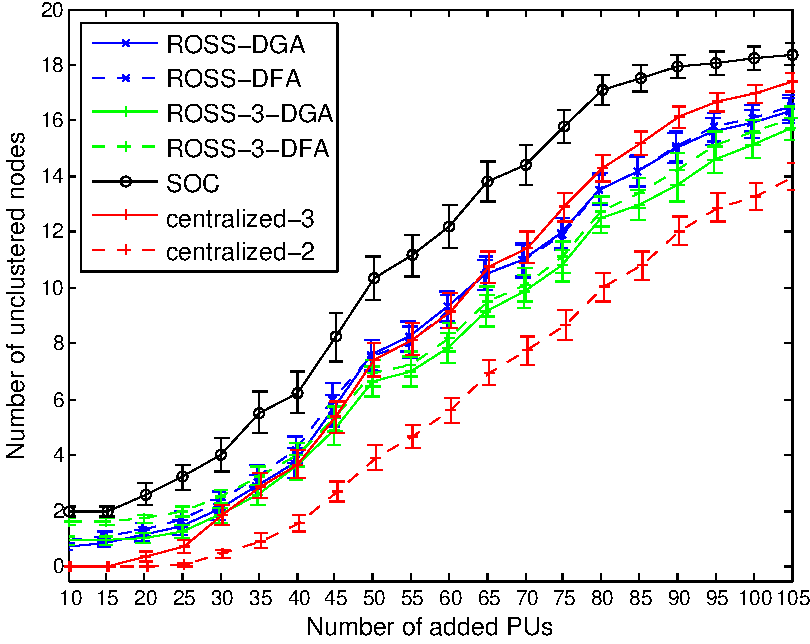
\includegraphics[width=\linewidth]{survival_rate_20.pdf}\par\caption{Number of CRs which are not included in any clusters}\label{singleton_clusters}
    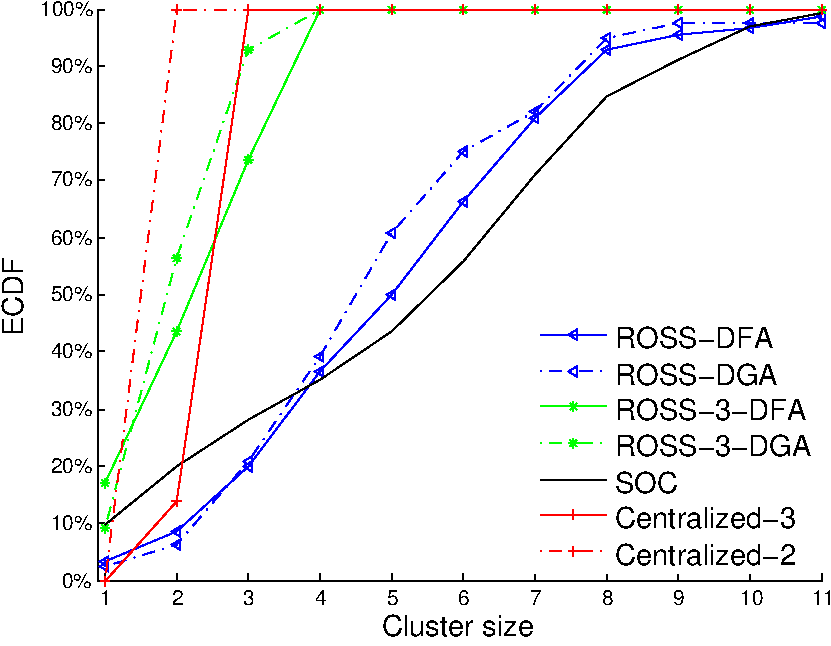
\includegraphics[width=\linewidth]{cdf_clusterSize_20.pdf}\par\caption{Cumulative distribution of CRs residing in clusters with different sizes}\label{size_control}
\end{multicols}
\caption{Comparison between the distributed and centralized clustering schemes in a small network ($N$ = 20)}
\label{compare_dis_centralized}
\end{figure*}


Figure~\ref{size_control} depicts the empirical cumulative distribution of the CRs residing in certain sized clusters in 50 runs.
The centralized schemes are able to form clusters which satisfy the requirement on cluster sizes strictly.
When the desired size is 2, each generated cluster has two members, whereas when the desired size is 3, about 15\% CRs are formed into 2 node clusters.
Both of ROSS-DFG and ROSS-DFA with size control feature also obtain clusters with homogeneous sizes.
%When ROSS-3-DFA is applied, most number of CRs are in 3 node clusters, nevertheless, slightly less nodes are found in 2 node and 4 node clusters, there are also considerable number of singleton clusters.
%ROSS-3-DGA decreases the clusters sizes and results in more 2 node clusters, the second most CRs are found in 3 node clusters.
The sizes of clusters generated by ROSS-DGA and ROSS-DFA are disperse, but appear better than SOC, i.e., the 50\% percentiles for ROSS-DGA, ROSS-DFA and SOC is 4.5, 5, and 5.5, and the 90\% percentiles for the three schemes are 8, 8, and 9.
%Figure~\ref{size_control} shows distributed clustering schemes are not able to control cluster sizes perfectly, but ROSS-DGA and ROSS-DFA eliminate the clusters whose size diverges largely with the desired one, \ie single node clusters and clusters with size of 13 and 14.
Note ROSS-DGA and ROSS-DFA with size control feature generate 10\%-20\% singleton clusters, which is due to the cluster pruning discussed in section~\ref{cluster_pruning}, whereas, without size control, only 3\% nodes are in singleton clusters.
When applying SOC, 10\% of nodes are in singleton clusters.

\subsubsection{Control Signalling Overhead}
%Different from the clustering schemes proposed in ~\cite{LIU_TMC11_2, clustering_globecom11}, 
%There are two phases for any variants of ROSS.
%Clusters are formed in the first phase, in the second phase, cluster membership is decided so that each node only resides in one cluster.
%Control message exchanges between CR nodes are involved in both phases.

In this section we compare the amount of control messages generated in different clustering schemes, \eg centralized scheme, ROC, and the variants of ROSS.

In order to highlight the amount of control signalling only for clustering, we omit the process of neighbourhood discovery, which is premise for all clustering schemes.
According to~\cite{complexity_aggregation_2011}, the message complexity is defined as the number of messages used by all nodes.
To have the same criterion to compare the overhead of signalling, we count \textit{the number of transmissions of control messages}, without distinguishing they are sent with broadcast or unicast.
This metric is Synonymous with \textit{the number of updates} discussed in Section~\ref{ross}.

As to ROSS, the control messages are generated in both phases.
In the first phase, %every CR node decides whether it is cluster head by comparing its spectrum robustness with its neighbours.
When a CR node decides itself to be the cluster head, it forms one cluster with its neighbourhood, 
each cluster head broadcasts one message containing its ID, cluster members and the set of CCCs in its cluster.
%As to ROSS with size control feature, there are same amount of cluster heads with ROSS without enabling size control feature, and the cluster head broadcasts the available channels of the pruned cluster.
In the second phase, %membership clarification of debatable nodes is conducted.
debatable node informs its claiming clusters by broadcasting its affiliation, and the claiming cluster's cluster head broadcasts message about its new cluster if its cluster's members are changed.
The total number of times for all CR nodes to send control messages, \ie the total number of decisions related with clustering functionality, has been analysed in the part of convergence speed in Theorem~\ref{clustering:theorem} and Section~\ref{clustering:phaseII:game} respectively.

Comparison scheme SOC involves three rounds of execution. 
In the first two rounds, every CR node maintains its own cluster and seek to integrate neighbouring clusters, or join in one of them.
The final clusters are obtained in the third round. 
In each round, every CR node is involved in comparisons and cluster mergers.
%Comparing with the second phase of ROSS, only debatable nodes to communicate with cluster heads to clarify their membership.
%The signalling overhead for centralized scheme comes from two processes, the the process of collecting information to the centralized controller, and the process that the controller spreads the clustering result to all the CR nodes.

As to the centralized scheme, except for the calculation in the centralized control device, it also involves two phases of control message transmission.
The first phase is information aggregation, in which every CR node's channel availability and neighbourhood is sent to the centralized controller.
The second phase is broadcasting, where the final clustering solution is disseminated over the network to every CR node.
%As basic communication primitive for wireless networks, 
We adopt the algorithm proposed in~\cite{Efficient_broadcasting_gathering_adhoc} to broadcast and gather information as the algorithm is simple and self-stabilizing.
This scheme needs building a backbone structure to support the communication, we use our generated cluster heads as the backbone and the debatable nodes as the gateway nodes between the backbone nodes.
As the backbone is built once and can support transmission for multiple times, the messages involved in the clustering process are not included.
Every CR node can be informed if the cluster heads broadcast the message sent from the controller or other cluster heads, then the number of transmission is $h+m$.
As to information gathering, we assume that every cluster member sends the spectrum availability and its ID to its cluster head, which further forwards or the message to the controller.
The number of transmission for information gathering is $N$.
%As we adopt a simplified communication model, node's transmission is not influenced by collision or interference, 
%Our simulation doesn't consider the behaviour in the physical layer, 
The number of transmission is depicted in Figure~\ref{control_msg}.
Note that the curve for the centralized scheme is from theoretical analysis, which is $h+m+N$ as discussed beforehand.
Note the overhead involved to construct the backbone (clusters) is not included.
%Assume we use OSPF~\cite{BCJ10} to aggregate and disseminate information, then the best and worst complexity for is $\mathcal{O}(E)$, where $E$ is the number of edges in the graph which corresponds to the network.
%The minimum number of edges is $n-1$ when the nodes form a line and each node has at more two neighbours, and the maximum number is $N*(N-1)/2$ when the nodes form a complete graph.
%Thus the best message complexity of the centralized scheme is $\mathcal{O}{(N)}$ and the worst is $\mathcal{O}{(N^2)}$.

%1. update membership to form X1, 
%2. broadcast new X1, form new X2
%3. broadcast X3

%The complexity parameters are the number of nodes $n$ in network, number of clusters $h$.
The message complexity, quantitative analysis of the number of messages, and the size of control messages are shown in Table \ref{tab_overhead}.
Some notations are written as follows,  $h$: number of cluster heads, $m$: number of debatable nodes, $d$: number of demanding clusters, $D(s)$: the maximum distance between centralized controller and CR users.

%\begin{table}[hc]
%\centering
%\caption{Singalling overhead. Notations: $n$-number of CR nodes in CRN, $h$-number of cluster heads, $m$-number of debatable nodes, $c$-number of demanding clusters.}\label{tab_overhead}
%\begin{tabular}{|p{2.2 cm}|p{1.5 cm}|p{3.7 cm}|}
%\hline
% Scheme 					&   Number of transmissions 					& Content of message \\ \hline
% ROSS-DGA, ROSS-x-DGA 		&   $h+2*m^2c$ (upper bound)
%				& $ID_{H_C}$ and $V_C$ for $h+m^2c$ times, notification to join in one cluster for $m^2c$ times					\\ \hline
% ROSS-DFA, ROSS-x-DFA 		&   $h+ 2m$	 (upper bound) 						& $ID_{H_C}$ and $V_C$ for $h+m$ times, notification to join in one cluster for $m$ times	 					\\ \hline
% SOC 						&   $3*n$					& $\{V_i\}, i\in M\subseteq \texttt{Nb}_i$						\\ \hline
% Centralized				&	$n$						& $\{C\}$         	\\ 
% \hline
%\end{tabular}
%\end{table}

\begin{center}
\begin{table*}[ht]
\caption{Singalling overhead.}\label{tab_overhead}
{\small
\hfill{}
\begin{tabular}{|L{2.2 cm}|C{2.8 cm}|C{3.15 cm}|C{6.6 cm}|}
\hline
 Scheme 				&Message Complexity 	&   Quantitative number of messages 		& Content of message 									\\ \hline
 ROSS-DGA, ROSS-x-DGA 	&$\mathcal{O}(N^3)$ (worst case)		&   $h+2*m^2d$ (upper bound)  				&   \multirow{2}{*}{\parbox{6.4cm}{Phase I: notification from cluster head (1 byte), new individual connectivity degree (1 byte);  Phase II: update of debatable nodes' affiliation (1 byte), claiming clusters' new membership ($|C_i|$ bytes)}}								\\ \cline{1-3}
 ROSS-DFA, ROSS-x-DFA 	&$\mathcal{O}(N)$ (worst case)		&   $h + 2m$	 (upper bound) 					& 	      												\\ \hline
 SOC 					&$\mathcal{O}(N)$		&   $3*N$									& $C_i$ ($|C_i|$ bytes), $V_i$ ($P$ bytes), $i\in \mathcal{N}$						\\ \hline
 Centralized			&$\mathcal{O}(N)$			&	$h + m + N$ (upper bound)~\cite{Efficient_broadcasting_gathering_adhoc}		& $\{C\}$ ($|C_i|*N$ bytes)        					\\ \hline
\end{tabular}
}
\hfill{}
\end{table*}
\end{center}
% centralized: $\mathcal{O}(D(s)+log N)$ + $\mathcal{O}(1+D(s)+log N)$



\begin{figure}[ht!]
  \centering
  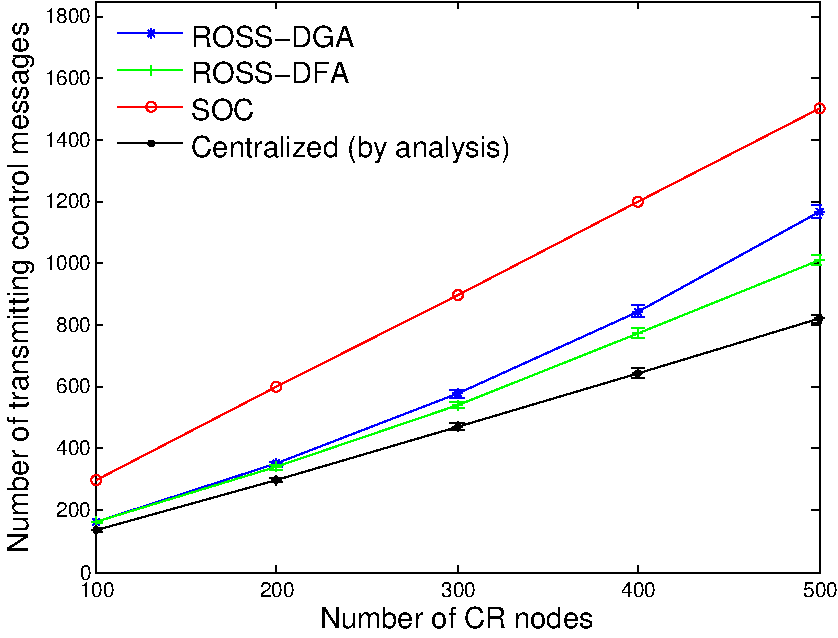
\includegraphics[width=0.7\linewidth]{number_controlMsg.pdf}
  \caption{Number of control messages, note the curves for ROSS-DGA and ROSS-DFA are the upper bounds of the number of messages, the curve of centralized scheme reflects an ideal situation.}
  \label{control_msg}
\end{figure}


\subsection{Comparison between Distributed Schemes}
In this section we investigate the performances of distributed clustering schemes in CRN with different network scales and densities.
The transmission range of CR is $A/10$, PR's transmission range is $A/5$.
The number of PU is 30.
%The number of CR is 100, 200 and 300, and the average number of neighbours of each CR is 9.5, 20, and 31.
We list some parameters of the simulation in the Table~\ref{Simulation_para}.


\begin{table}[ht]
\caption{}
\label{Simulation_para}
{\small
\hfill{}
\begin{tabular}{|L{3.7 cm}|C{1 cm}|C{1 cm}|C{1 cm}|}
\hline
Number of CRs			& 100 	&  200 					& 300 \\ \hline
Average num. of neighbours 	&9.5	&   20		& 31  \\ \hline
Desired size $\delta$ 	& 6	&   12 						& 20      \\ \hline
\end{tabular}
}
\hfill{}
\end{table}



\subsubsection{Number of CCCs per Non-singleton Clusters}

\begin{figure}[ht!]
  \centering
  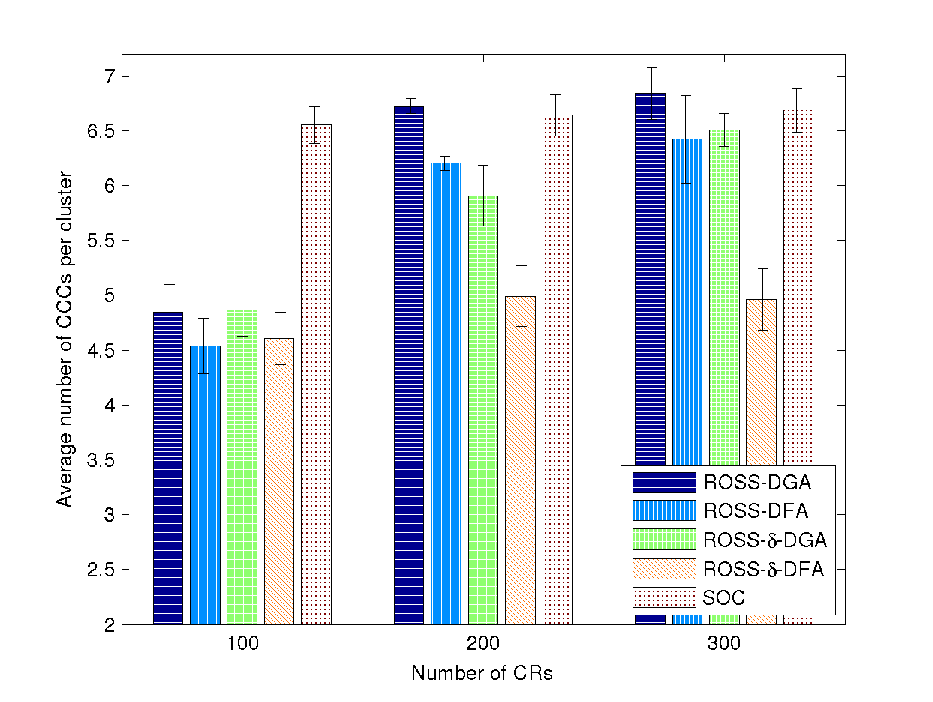
\includegraphics[width=1\linewidth]{ccc_large_scale_color.pdf}
  \caption{Number of common channels of non-singleton clusters.}
  \label{ccc_large_scale}
\end{figure}

Figure~\ref{ccc_large_scale} illustrates the average number of CCCs of the non-singleton clusters.
It shows when $N=100$, variants of ROSS have 30\% less CCCs than SOC, but this gap is decreased significantly when $N$ is 200 and 300, \ie when $N=300$, number of CCCs achieved by ROSS variants (except for ROSS-x-DFA) is almost the same with that resulted from SOC.

This means SOC performs better in terms of the average number of CCCs per non-singleton clusters when network is sparse.
this is also observed in the evaluation in Section \ref{ccc_20} where $N=20$.
When the network becomes denser, even this metric favours SOC as discussed in the beginning of Section~\ref{performance}, ROSS-DGA achieves even more CCCs than SOC, and ROSS-DFA and ROSS-x-DGA increase the number of CCCs visibly.




\subsubsection{Survival Rate of Clusters with Increasing Primary Users}

In this part of simulation, we investigate the robustness of clusters by increasing the PUs working on certain channels.
 
Figure~\ref{singleton_clusters_100} illustrates the increasing trend of singleton clusters with the increase of PUs.
SOC generates around 10 more singleton clusters than the variants of ROSS, which accounts for 10\% of the total CR nodes.
We only show the average values of the variants of ROSS as their confidence intervals overlap.
%It can be seen that greedy algorithms result in slightly less singleton clusters than their counterparts.
%
Figure ~\ref{singleton_clusters_300} depicts a denser CRN where $N=300$.
SOC noticeably causes more singleton clusters than ROSS variants, except that ROSS-20-DFA results in more singleton clusters when PUs are few.
The reason is ROSS-20-DFA conducts cluster membership clarification for only once, which causes large number of singleton clusters.
ROSS-20-DGA increases the size of smaller clusters through debatable nodes' repeated updates thus drastically decreases the number of singleton clusters.

\begin{figure}[!h]
  \centering
  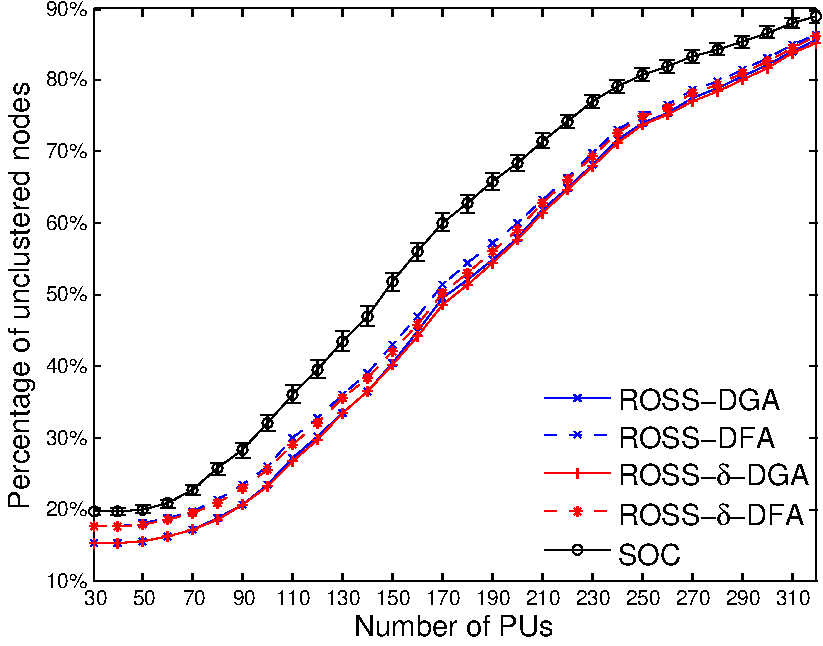
\includegraphics[width=0.8\linewidth]{survival_rate_100.pdf}
  \caption{Percentage of CRs which are not included in any clusters with the increasing number of primary users, $N=100$}
  \label{singleton_clusters_100}
\end{figure}
  
  \begin{figure}[!h]
    \centering
   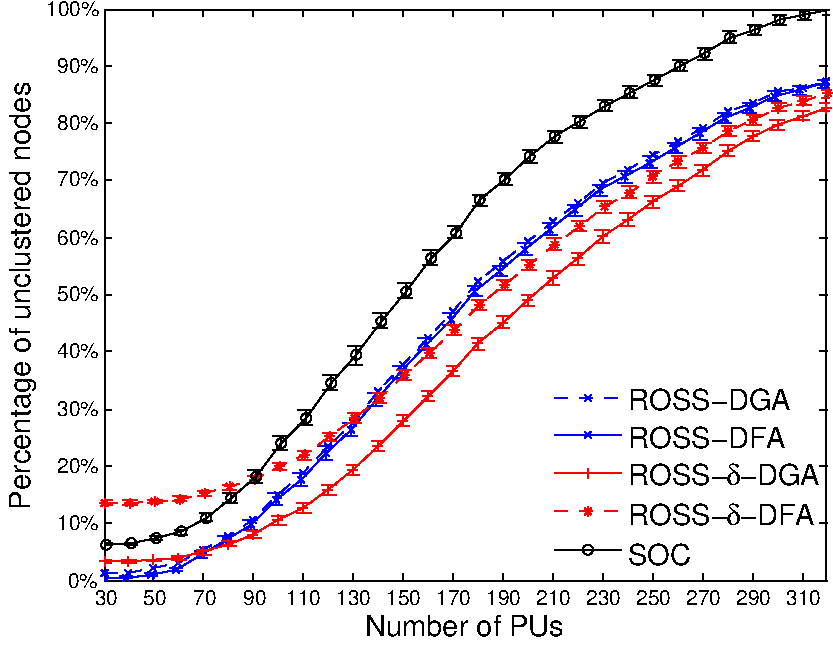
\includegraphics[width=0.8\linewidth]{survival_rate_300.pdf}
  \caption{Percentage of CRs which are not included in any clusters with the increasing number of primary users, $N=300$}
  \label{singleton_clusters_300}
\end{figure}

From the Figure~\ref{singleton_clusters_100} and \ref{singleton_clusters_300}, we can conclude that the greedy versions of ROSS are slightly more robust than their counterpart variants of ROSS, and the clusters obtained from variants of ROSS are clearly more robust than SOC. 
%When the network is denser, the improvement on cluster sizes and robustness by the greedy search in the membership clarification phase is more obvious.


\subsubsection{Cluster Size Control}

The number of formed clusters is shown in Fig.~\ref{nClusters_largeNetwork}.
When the network scales up, the number of formed clusters by ROSS increases by smaller margin.
This result coincides with the analysis in Section~\ref{cluster_pruning}, that with ROSS, the number of formed clusters saturates when the network scales.
When the network becomes denser, more clusters are generated by SOC compared with ROSS variants.
To better understand the distribution of the sizes of formed clusters, we depict the cluster sizes with cumulative distribution.
In this group of evaluation, the number of PRs is 30.

\begin{figure}[!h]
  \centering
   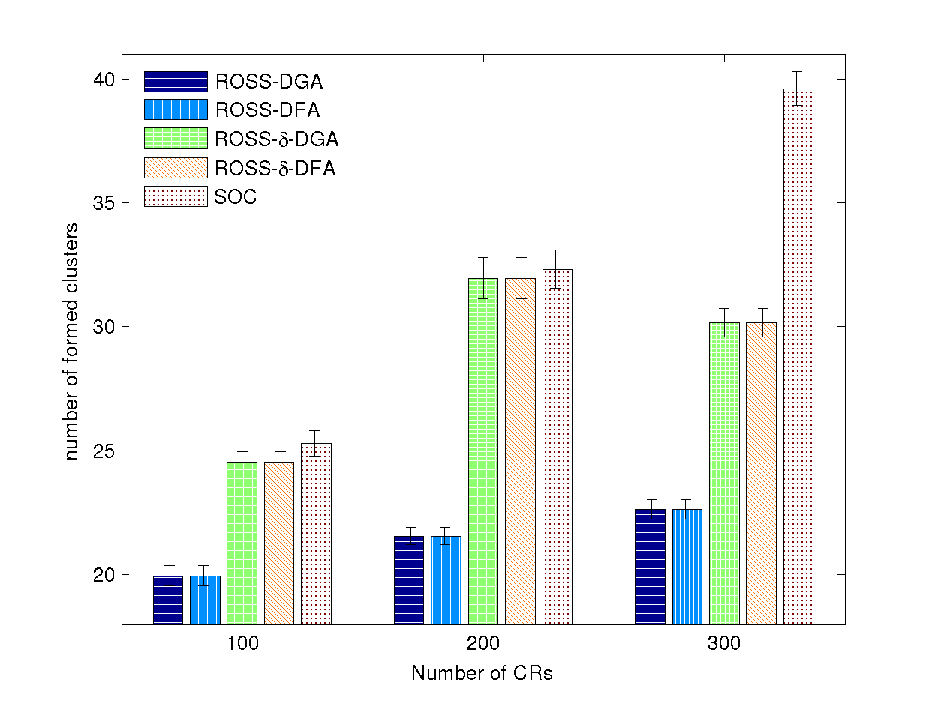
\includegraphics[width=1\linewidth]{nClusters_largeNetwork.pdf}
  \caption{The number of formed clusters.}
  %, there are $x=6$ when $N=100$, $x=12$ when $N=200$, $x=21$ when $N=300$, which is around $2/3$ of the number of average neighbours.
  \label{nClusters_largeNetwork}
\end{figure}





%\begin{figure}[ht]
%\begin{center}
%%\centering
%\subfigure[100 CRs, 30 PRs]{\label{result1:1}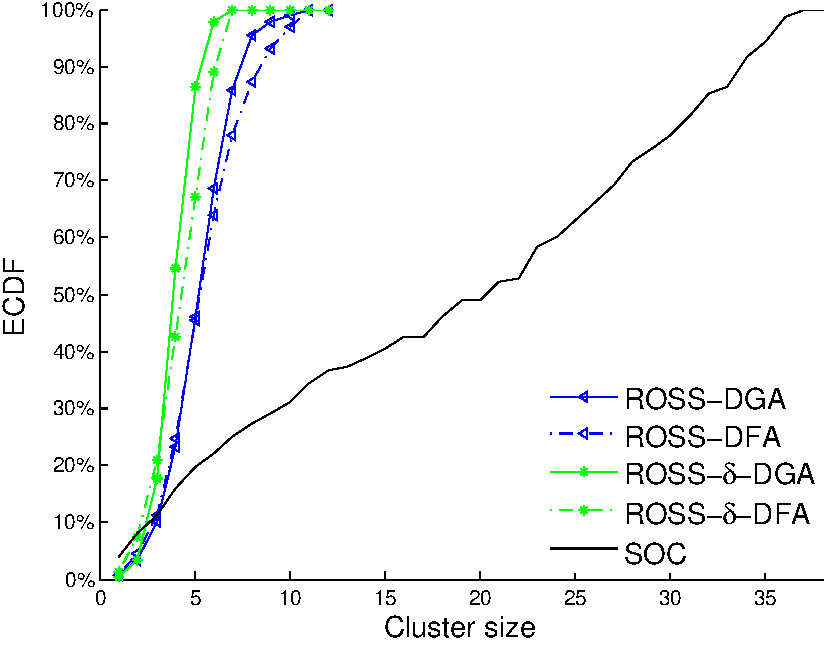
\includegraphics[width=0.48\linewidth]{cdf_clusterSize_100.pdf}}
%\subfigure[300 CRns, 30 PRns]{\label{result1:2}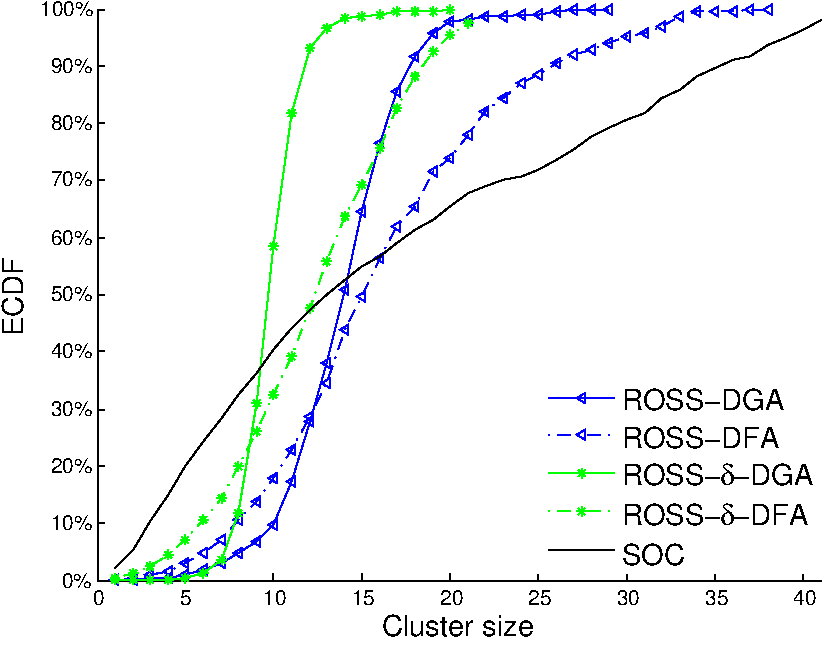
\includegraphics[width=0.48\linewidth]{cdf_clusterSize_300.pdf}}
%\end{center} 
%\caption[Cluster sizes]{Distribution of CRs in clusters with different sizes} %{\subref{a}, \subref{b}, \subref{c}, \subref{d}}
%\label{result1}
%\end{figure}

Figures~\ref{cdf_clusterSize_100}~\ref{cdf_clusterSize_200}~\ref{cdf_clusterSize_300} illustrate the empirical cumulative distribution of CR nodes which reside in clusters with certain sizes in CRNs with different densities.
%The desired cluster sizes are 5, 8 and 13, which are around 45\% of the average number of neighbours in respective CRNs. 
When the variants of ROSS with size control feature are applied, the sizes of the most generated clusters are below $\delta$, and most of them are around the 50\% percentile.
%This means the size control feature effectively restricts the size of clusters, which is able to prevent the clusters from ungovernable growing with the increase of network density.
The sizes of clusters generated by ROSS-DGA and ROSS-DFA span a wider range than that with feature control feature.
We find that average number of neighbours is roughly equal with the 95\% percentile of the ROSS-DGA curve.
%But the range where most of the CRs (80\% which exclude the CR nodes residing in small and big clusters) resides centres a value, which is roughly the half of the average number of neighbours.
As to SOC, the 95\% percentiles are 36, 30, and 40.
Overviewing the three Figures, we can see ROSS-DGA and ROSS-DFA show similar behaviour on cluster sizes.
The clusters generated from SOC demonstrate strong divergence on cluster sizes.


\begin{figure*}[t]
\begin{multicols}{3}
    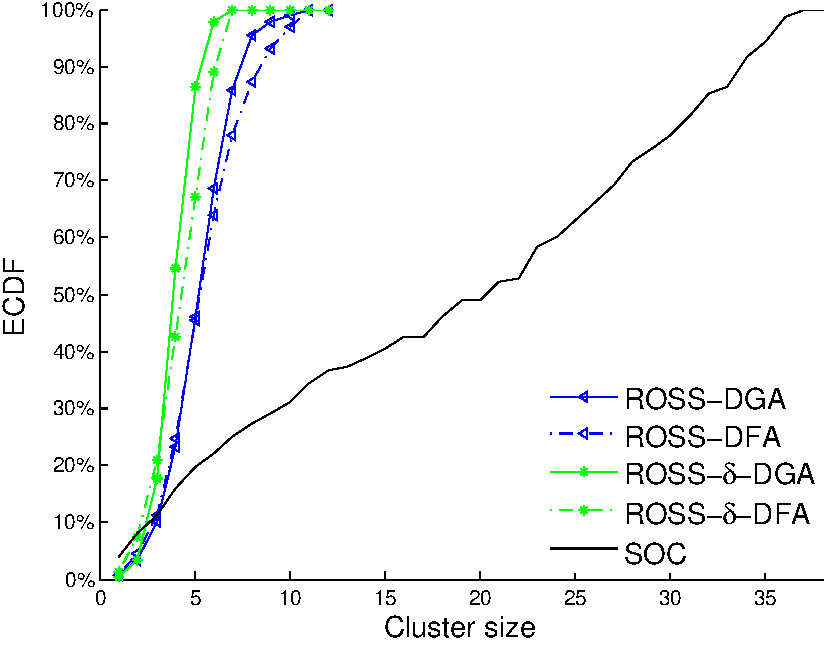
\includegraphics[width=\linewidth]{cdf_clusterSize_100.pdf}\par\caption{100 CRs, 30 PRs in network}\label{cdf_clusterSize_100}
    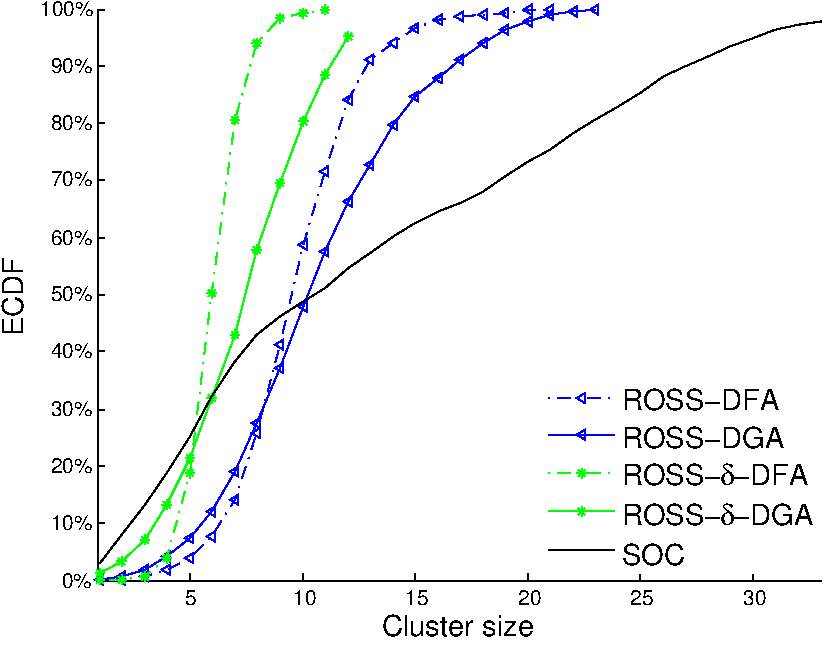
\includegraphics[width=\linewidth]{cdf_clusterSize_200.pdf}\par\caption{200 CRs, 30 PRs in network}\label{cdf_clusterSize_200}
    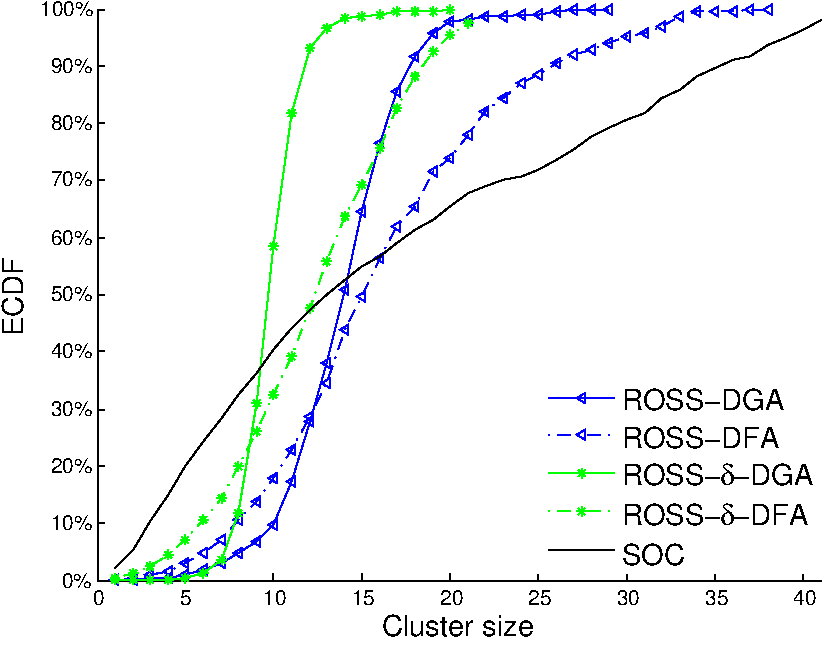
\includegraphics[width=\linewidth]{cdf_clusterSize_300.pdf}\par\caption{300 CRs, 30 PRs in network}\label{cdf_clusterSize_300}
\end{multicols}
\caption{Cumulative distribution of CRs residing in clusters with different sizes}
\label{cdf_100_200_300}
\end{figure*}


\section{Conclusion}
\label{conclusion}
In this paper we design a distributed clustering scheme with the singleton congestion model, which forms robust clusters against primary users' effect.
Through simulation and theoretical analysis, we find that distributed scheme achieves similar performance with centralized optimization in terms of cluster survival ratio and number of control messages.
%, which is important to form clusters which maintains unbroken to the greatest extent possible under primary users' activity.
This paper investigates the robust clustering problem in CRN extensively, and proves the NP hardness of this problem.
A Light weighted clustering scheme ROSS is proposed, on the basis of which, we propose the fast version scheme and the scheme which generate clusters with desired sizes.
These schemes outperform other distributed clustering scheme in terms of both cluster survival ratio and control overhead.

%The clusters resulted from ROSS-DGA and its faster version ROSS-DFA are less vulnerable compared with other distributed clustering schemes, and demonstrates similar survival rate with centralized scheme under primary users' influence.
%An light weighted cluster size control mechanism is contained in both ROSS-DGA and ROSS-DFA, which is advantageous for cooperative sensing and network operation with clusters.
%Furthermore, considerable less control messages are generated when compared with other clustering schemes.

The shortage of ROSS scheme is it doesn't generate big clusters whose sizes exceed the cluster head's neighbourhood.
This problem is attributed to fact that ROSS forms clusters on the basis of cluster head's neighbourhood, and doesn't involve interaction with the nodes outside its neighbourhood.
In the other way around, forming big cluster which extends out side of cluster head's neighbourhood has very limited applications, because multiple hop communication and coordination are required mange this kind of big clusters.








% if have a single appendix:
%\appendix[Proof of the Zonklar Equations]
% or
%\appendix  % for no appendix heading
% do not use \section anymore after \appendix, only \section*
% is possibly needed

% use appendices with more than one appendix
% then use \section to start each appendix
% you must declare a \section before using any
% \subsection or using \label (\appendices by itself
% starts a section numbered zero.)
%


\appendices
%\section{Algorithm~\ref{alg0}}
\section*{}
\begin{algorithm}              % enter the algorithm environment
\caption{ROSS phase I: cluster head determination and initial cluster formation for Unclustered CR node $i$}          % give the algorithm a caption
\label{alg0} 
\DontPrintSemicolon
\SetAlgoLined
\KwIn{$D_j, G_j, j\in \texttt{Nb}_i\setminus CHs$. Empty sets $\tau_1,\tau_2$}
\KwResult{1 means $i$ is cluster head, then $D_j, j\in \texttt{Nb}_i\setminus CHs$ is changed as a big positive value $M$. 0 means $i$ is not.}

\If{$\nexists j\in \texttt{Nb}_i\setminus CHs$, such that $D_i \leq D_j$}{
	return 1;
	}
\eIf{$\exists j\in \texttt{Nb}_i\setminus CHs$, such that $D_i < D_j$}{
	return 0;}{
	\If{$\nexists j\in \texttt{Nb}_i\setminus CHs$, such that $D_j == D_i$}{
	$\tau_1 \leftarrow j$
	}
}
\If{$\nexists j\in \tau_1$, such that $G_i \leq G_j$}{
	return 1;
	}
\eIf{$\exists j\in \tau_1$, such that $G_i < G_j$}{
	return 0;
	}
	{\If{$\nexists j\in \tau_1$, such that $G_j == G_i$}{
		$\tau_2\leftarrow j$
		}
	}
\If{$\texttt{ID}_i$ is smaller than any $\texttt{ID}_j$, $j\in \tau_2\setminus i$}{
	return 1;
	}
	{return 0;
	}
\end{algorithm}

% you can choose not to have a title for an appendix
% if you want by leaving the argument blank
%\section*{Algorithm~\ref{alg_size_control_available_CCC}}
\section*{}
\begin{algorithm}               % enter the algorithm environment
\caption{ROSS phase I: cluster head guarantees the availability of CCC (use line 1) / cluster size control (use line 2)}          % give the algorithm a caption
\label{alg_size_control_available_CCC}
\DontPrintSemicolon
\SetAlgoLined
\KwIn{Cluster C, empty sets $\tau_1, \tau_2$}
\KwOut{Cluster C has at least one CCC, or satisfies the requirement on cluster size}
%\tcc*[r]{When to guarantee available CCCs, execute from line 1, when to control cluster size, execute from line 2}
\textbf{while} $V_C =\emptyset$ \textbf{do}\\
\While{$|C|> \delta$}{
	%calculate $\lambda = \min_{i\in C, i\neq H_C}(|K_{H_C}\cap K_i|)$;\\
	\eIf{$\exists$ only one $i\in C\setminus H_C$, $i = \argmin(|K_{H_C}\cap K_i|)$}{
			$C=C\setminus i$;
		}{
				$\exists$ multiple $i$ which satisfies $i = \argmin(|K_{H_C}\cap K_i|)$;\\ $\tau_1\leftarrow i$;		
		}
		
	\eIf{$\exists$ only one $i\in \tau_1$, $i = \argmax(|\cap_{j\in C\setminus i} V_j|-|\cap_{j\in C} V_j|)$}{
		$C=C\setminus i$;
		}{
			%$\exists$ multiple $i$ which satisfies $i = \argmax(|\cap_{j\in C\setminus i} V_j|-|\cap_{j\in C} V_j|)$;\\
			$C=C\setminus i$, where $i = \argmin_{i\in \tau_1} \texttt{ID}_i $
			%$\texttt{ID}_i$ is smaller than any $\texttt{ID}_j$, $j\in \tau_2\setminus i$;
	}
}
\end{algorithm}


\section*{}
\begin{algorithm}               % enter the algorithm environment
\caption{Debatable node $i$ decides its affiliation in phase II of ROSS}
%, chooses one claiming cluster to stay and leaves all the other claiming clusters}          % give the algorithm a caption,  cluster to settle
\label{alg4}
\DontPrintSemicolon
\SetAlgoLined
\KwIn{all claiming clusters $C\in S_i$}
\KwOut{one cluster $C\in S_i$, node $i$ notifies all its claiming clusters in $S_i$ about its affiliation decision.
}
\While{$i$ has not chosen the cluster, or $i$ has joined cluster $\tilde{C}$, but $\exists C'\in S_i, C'\neq \tilde{C}$, which has $|K_{C'\setminus i}|-|K_{C'}|<|K_{C\setminus i}|-|K_{C}|$}{
	\eIf{$\exists$ only one $C\in S_i$, $C = \argmin(|K_{C\setminus i}| - |K_C|)$}{
			return $C$;
		}{
				$\exists$ multiple $C\in S_i$ which satisfies $C = \argmin(|K_{C\setminus i}| - |K_C|)$;\\ 
				$\tau_1\leftarrow C$;		
		}
	\eIf{$\exists$ only one $C\in \tau_1$, $C = \argmax(V_{H_C}\cap V_i)$}{
			return $C$;
		}{
				$\exists$ multiple $C\in S_i$ which satisfies $C = \argmax(V_{H_C}\cap V_i)$;\\ 
				$\tau_2\leftarrow C$;		
		}
	\eIf{$\exists$ only one $C\in \tau_2$, $C = \argmin|C|)$}{
			return $C$;
		}{
				return $\argmin_{C\in \tau_2}\texttt{ID}_{H_C}$;\\
		}
		}
\end{algorithm}

% use section* for acknowledgment

\section*{Proof of Theorem~\ref{clustering:theorem}}
\label{proof_clustering:theorem}
\begin{proof}
Note the formed cluster can be a singleton cluster, \ie cluster size is 1.
To simplify the proof, we assume secondary users have unique individual connectivity degrees.
This is fair as there are other metrics to break the tie according to Algorithm~\ref{alg0}, \ie the social connectivity degrees and node ID.
Assuming there are some secondary users which are not assigned to any cluster and node $\alpha$ is one of them.
As node $\alpha$ is not contained in any cluster, there must be at least one node $\beta\in Nb_\alpha$, with $D_{\alpha} < D_{\beta}$.
Otherwise, node $\alpha$ is eligible to form a cluster.
Then, as node $\beta$ form a cluster and include node $\alpha$, we can repeat the analysis on node $\alpha$, and deduce that node $\beta$ has at least one neighbouring node $\gamma$ with $D_{\gamma}>D_{\beta}$, and this series of nodes with monotonically increasing $D_i$ might continue to grow and ceases finally because both of the individual connectivity degree 
and the total number of nodes are limited.
The formed node series is shown as Figure~\ref{lemma1}.

\begin{figure}[ht!]
  \centering
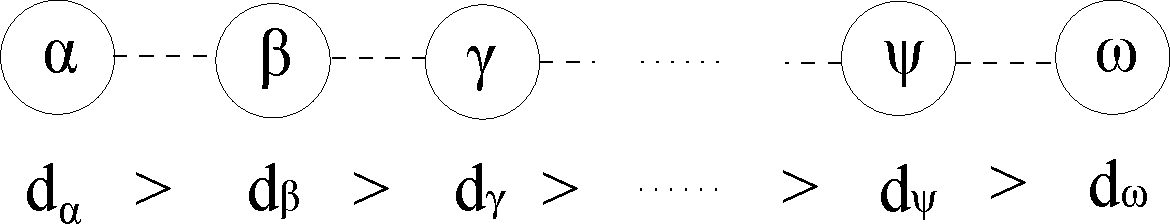
\includegraphics[width=0.6\linewidth]{lemma1.pdf}
% 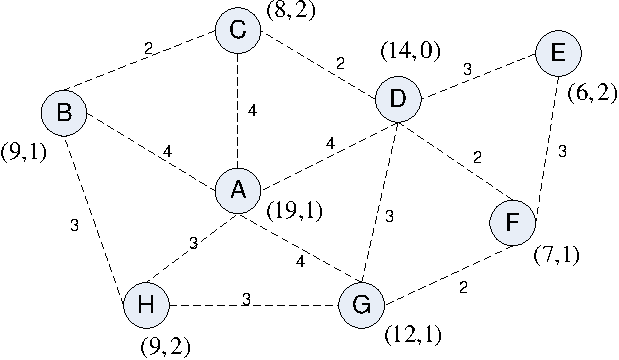
\includegraphics{figure1.pdf}
	\caption{The node series discussed in the proof for Theorem~\ref{clustering:theorem}, the deduction begins from node $\alpha$}
	\label{lemma1}
\end{figure}


Now we find the node $\omega$ is in the end of this series.
As $\omega$ is the end node and does not have neighbouring nodes with bigger individual connectivity degree $D$, $\omega$ becomes cluster head and incorporate all its one-hop neighbours, including the node before it in the node series (here we assume that every new formed cluster has common channels).
After that, the node recruited into cluster will set its connection degree $D$ to zero, which enables the node further down in the list to become a cluster head.
In this way, all the nodes in the series are included in at least one cluster in an inverse sequence.
This result contradicts the initial assumption and proves the claim stated above.
Meanwhile, through this proof, we know that within at most $N$ steps, all nodes will become a part of certain clusters.
\end{proof}


%
\section*{Proof of Theorem~\ref{theorem1}}
\label{proof_theorem1}
\begin{proof}
We put the definition of weighted k-set packing problem here as it will be used in the analysis on the complexity of our problem.

\begin{mydef}
\label{def_kset_packing}
\textit{Weighted k-set packing.} 

Given a set $\mathcal{G}$ which contains finite number of positive integers, and a collection of set $\mathcal{Q}=\{s_1,s_2,\cdots,s_m\}$, where for each element $s_r, 1\leq r \leq m$, there is $s_r\subseteq \mathcal{G}$, $ 1\leq|s_r| \leq k$, and $s_r$ has an associated weight which is positive real number.
The question is whether exists a collection $\mathcal{S}\subseteq \mathcal{Q}$, where $\mathcal{S}$ contains only disjoint sets and the total weight of sets in $\mathcal{S}$ is greater than $\lambda$.
Weighted k-set packing is NP-hard when $k\geqslant 3$.~\cite{Computers_a_Intractability}
\end{mydef}


To prove the centralized clustering problem is of NP-hard, we reduce the NP-hard problem \textit{weighted k-set packing} to it to prove the former is as hard as the later.
%, which means centralized clustering in CRN problem is as hard as weighted k-set packing to be solved.
To complete the reduction, we need to conduct following two steps:
\begin{itemize}
\item step 1: Show there exists a polynomial algorithm $\sigma$, by which any instance $\mathcal{S}$ of a weighted k-set packing can be transformed to a clustering solution $\sigma(\mathcal{S})$ which complies with Definition~\ref{def_centralized_clustering}.
\item step 2: Show that $\mathcal{S}$ is a \textit{yes} instance of weighted k-set packing if and only if $\sigma(\mathcal{S})$ is a \textit{yes} instance for CRN clustering problem.
\end{itemize}

We continue to use the notation adopted in the problem definition in Section~\ref{centralized_opt}.
Let set $\mathcal{G}$ contain $N$ natural numbers which are from 1 to $N$.
$\mathcal{Q}$ is a collection of sets $\{s_1, s_2,\cdots s_m\}$, each set is composed with certain elements in $\mathcal{G}$.
Assume $\mathcal{S}\subseteq \mathcal{Q}$ is one instance of weighted k-set packing, and the sets in $\mathcal{S}$ are disjoint.
$\omega$ indicates the weight for each set $s$, $\omega:\mathcal{S}\rightarrow \mathbb{Z}^{+}$.
%As the number of common channel of clusters is always integer
%give new weight to them in following way



The polynomial algorithm $\sigma$ consists of three transformations.

\begin{itemize}
\item Given a collection $\mathcal{Q}$, on basis of which we construct a CRN.
We prepare $N$ CR nodes who are labelled from 1 to $N$.
We put the CR users on a 2 dimension space, and deem a pair of them can communicate if they appear in the same set in $\mathcal{Q}$.
We regard each set in $\mathcal{Q}$ is a cluster, whose number of CCCs equals to the weight of that set.


%There is one situation deserving extra explanation in the second transformation, we adopt one example to discuss it.
Assuming two sets in $\mathcal{Q}$ are $s_1=\{1,2\}$ and $s_2=\{1,2,3\}$, then their weights are 3 and 5 respectively.
%Their dummy sets are $s_1'=\{1,1,2,2\}$ and $s_2'=\{1,1,2,2,3,3,4,4\}$ and their new weights are 3 and 5 as before.
We find it is impossible to map the sets into clusters in the same time, because the number of CCCs of the cluster which bases on $s_1$ should be no less than the cluster which bases on $s_2$, as the latter has one extra node compared with the former cluster.
%When $s_1'$ and $s_2'$ are mapped to CRN respectively, there is contradiction between them, because the number of common channels of CR node group $\{1,1,2,2\}$ is smaller than that of $\{1,1,2,2,3,3,4,4\}$.
But as to any instance of the solution to the weighted k-set packing problem, this contradiction doesn't happen because the instance $\mathcal{S}$ contains only disjoint sets, thus at most only one set of $s_1$ and $s_2$ appears in $\mathcal{S}$.%, then we can safely delete the connections based on the deleted set from the CRN, and the contradiction is eliminated.

\item In the second step, we transform the instance $\mathcal{S}$ to $\mathcal{S'}$ by adding dummy elements into each set in $\mathcal{S}$.
For each set $s_i\in \mathcal{S}$, the elements in $s_i$ are duplicated, for instance, given $s_i=\{1, 4, 6\}$, the dummy set $s_i'$ is $\{1,1,4,4,6,6\}$.
%By doing this, we obtain the dummy sets and constitute the dummy instance $\mathcal{S}'$ based on $\mathcal{S}$.
The purpose of this transformation is to eliminate the set in $\mathcal{S}$, which has single element.
The weight of set is unchanged after this transformation, \ie $\omega(s_i)=\omega(s_i')$.
%After this transmission, there is no set with only one element.
This transformation requires $\sum_{s_i \in \mathcal{S}} |s_i|$ steps.

\item In this step, we transform the instance $\mathcal{S'}$ to a clustering solution for CRN.
We prepare a second pool of CR nodes which are identical with the CR nodes prepared in step 1, i.e., identical IDs and channel availabilities on them, we call these CR nodes as dummy nodes.
We locate these CR nodes besides the CR nodes with the sane IDs in the CRN built in step 1, and there is connection between the CR node and its dummy node (the one CR node and its dummy node can be seen as two transceivers at one node).
Because of the dummy nodes, the clustering solution which corresponds to $\mathcal{S'}$ doesn't have singleton cluster.
This transformation requires $2\cdot\sum_{s_i \in \mathcal{S}} |s_i|$ steps.
%
Afterwards, the CR node whose ID doesn't appear in any set in $\mathcal{S}$ becomes single node clusters, according to the definition of clustering problem in CRN, the number of CCCs in these single node clusters is 0.
These singleton clusters and the clusters in $\mathcal{S}$ constitute a clustering solution, and finding the singleton clusters requires at most $N$ steps.
%We deliberately locate them so that at least one CR node can communicate with the rest of them.
%map every element in $\mathcal{S}$ into one CR node, \ie each integer corresponds to one CR node, in particular, that integer becomes the CR node's ID.
%As $s'$ is dummy set which has duplicated elements, we also deploy the the same CR node twice.

An example is shown in Table~\ref{no_hard_proof_instance}.
\begin{table}[h!]
     \begin{center}
     \begin{tabular}{ p{3cm}  p{4.5cm} }
     \toprule
      $\mathcal{N}$  & $\{1,2,3,4,5\}$\\ 
    \cmidrule(r){1-1}\cmidrule(lr){2-2}     
      $\mathcal{Q}$  & $\{(1),(1, 5),(1,2,4),(2,3), (4)\}$\\ 
    \cmidrule(r){1-1}\cmidrule(lr){2-2}     
      Instance for Weighted k-set packing  & $\{(1),(2,3), (4)\}$\\ 
    \cmidrule(r){1-1}\cmidrule(lr){2-2}
      Instance with dummy elements
      & 
		$\{(1,1),(2,2,3,3), (4,4)\}$
      \\    \cmidrule(r){1-1}\cmidrule(lr){2-2}
	Instance for clustering solution (dashed circles are dummy nodes)
	  &
	  %\raisebox{-\totalheight}{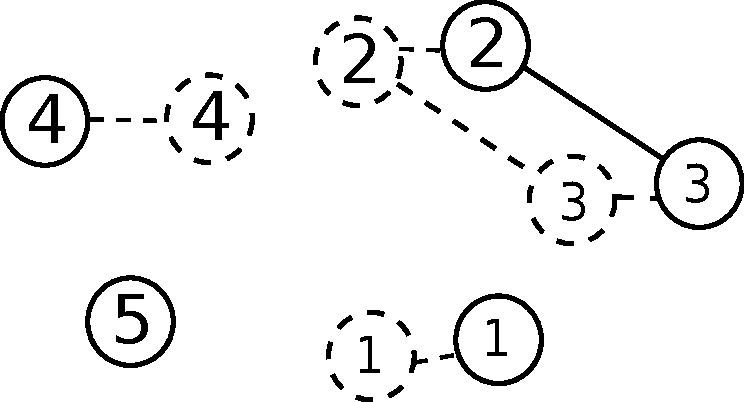
\includegraphics[width=0.8\linewidth]{np_hard_proof_dummy.pdf}}      
	  \begin{minipage}{.3\textwidth}
      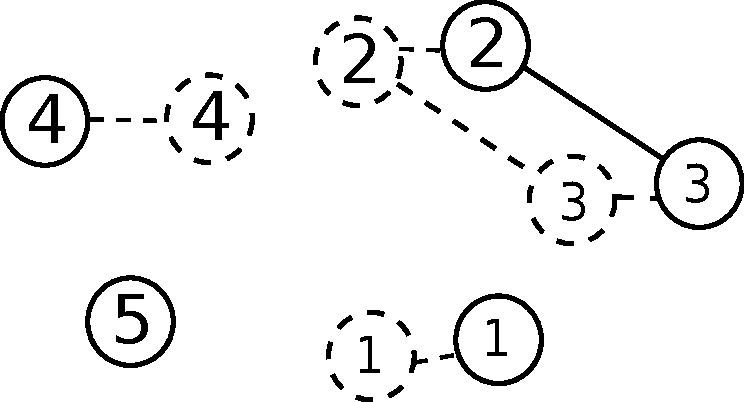
\includegraphics[width=0.8\linewidth]{np_hard_proof_dummy.pdf}
    \end{minipage}
	  \\       \bottomrule
      \end{tabular}
      \caption{}
      \label{no_hard_proof_instance}
      \end{center}
      \end{table}

%As to duplicated elements, we also map them into a CR node, thus there exist CR nodes with identical ID.
%As a result, these CR nodes constitute a collection of CR nodes, and they can not be called as a CRN yet as there are not communication links drawn between them.
%Connections in CRN under this context is decided by physical conditions, which means to have a communication link, the two CR nodes should have common channels and locate within each other's transmission range.
%We further assume that all CR nodes locate in a way that any two pair of nodes has potential to be connected if their IDs are in the same set in $\mathcal{S}$, the instance for weighted k-set packing.
%\item Mere isolated nodes don't constitute network, thus we add connections in CRN based on the sets in $\mathcal{S}'$ sequentially.
%For each set $s'\in \mathcal{S}'$, we add connection between two CR nodes if their IDs can be found in $s'$.
%No connection exists between two CR nodes if their IDs don't appear in the same set in $\mathcal{S}$.



%We complete the polynomial algorithm $\sigma$ for the the transformation so far.
%The number of common channels of cluster $f$ is non-increasing function of cluster size, while, the weight of set in weighted k-set packing problem doesn't have this property.
%In weighted k-set packing, the weight of a set with smaller size could be larger than a set with more elements.
%But this difference doesn't hinder the transformation because an instance of weighted k-set packing contains only disjoint sets in $\mathcal{G}$.

\end{itemize}

We have crossed the hurdle of finding one polynomial algorithm $\sigma$ to transform instance of weighted k-set packing to an instance for clustering in CRN.
Now we look into the step 2 in reduction.

As to an instance $\mathcal{S}$ for weighted k-set packing, the sum weights is identical to the sum of CCCs in the CRN mapped from $\mathcal{S'}$, even $\mathcal{S}$ contains set which only has one element.
Thus, when the instance $\mathcal{S}$ is one solution and its sum weights is greater than $\lambda$, in the CRN which is mapped from $\mathcal{S'}$, the summed number of CCCs of the clusters is greater than $\lambda$.
%
When there is no solution out of set $\mathcal{G}$ for weighted k-set packing,
%let's assume the maximum sum of weights of all instances is $\sum_{s_i\in \mathcal{S}}\omega(s_i)=\delta < \lambda$. 
%The dummy set of each $s_i\in \mathcal{S}$ is mapped to cluster of CR nodes.
%Definition of CRN clustering regulates that the number of common channels is 0 when the cluster has only one node.
%As to $|s_i|=1$, the mapped cluster has two nodes, with one of them is the dummy CR node.
%Then number of common channels is on longer 0 but equals to the weight of corresponding set $s_i$.
%%Meanwhile, the number of common channels of all the other single node cluster is 0.
the summed number of CCCs of the clusters in the mapped CRN is also smaller than $\lambda$.

Thus, weighted k-set packing can be reduced to centralized clustering problem in CRN, and we can say the latter problem is of NP-hard.
\end{proof}


\section*{Acknowledgment}

The authors would like to thank xxxx


% Can use something like this to put references on a page
% by themselves when using endfloat and the captionsoff option.
\ifCLASSOPTIONcaptionsoff
  \newpage
\fi



% trigger a \newpage just before the given reference
% number - used to balance the columns on the last page
% adjust value as needed - may need to be readjusted if
% the document is modified later
%\IEEEtriggeratref{8}
% The "triggered" command can be changed if desired:
%\IEEEtriggercmd{\enlargethispage{-5in}}

% references section

% can use a bibliography generated by BibTeX as a .bbl file
% BibTeX documentation can be easily obtained at:
% http://mirror.ctan.org/biblio/bibtex/contrib/doc/
% The IEEEtran BibTeX style support page is at:
% http://www.michaelshell.org/tex/ieeetran/bibtex/
%\bibliographystyle{IEEEtran}
% argument is your BibTeX string definitions and bibliography database(s)
%\bibliography{IEEEabrv,../bib/paper}
%
% <OR> manually copy in the resultant .bbl file
% set second argument of \begin to the number of references
% (used to reserve space for the reference number labels box)


% biography section
% 
% If you have an EPS/PDF photo (graphicx package needed) extra braces are
% needed around the contents of the optional argument to biography to prevent
% the LaTeX parser from getting confused when it sees the complicated
% \includegraphics command within an optional argument. (You could create
% your own custom macro containing the \includegraphics command to make things
% simpler here.)
%\begin{IEEEbiography}[{\includegraphics[width=1in,height=1.25in,clip,keepaspectratio]{mshell}}]{Michael Shell}
% or if you just want to reserve a space for a photo:

\begin{IEEEbiographynophoto}{Di Li}
received BE and MS degrees in control engineering from Zhejiang University and Shaanxi University of Science and Technology respectively in China.
He worked with James Gross for his PhD in RWTH Aachen University since 2010.
\end{IEEEbiographynophoto}

% if you will not have a photo at all:
\begin{IEEEbiography}{Erwin Fang}
Biography text here.
Biography text here.
Biography text here.
Biography text here.
Biography text here.
Biography text here.
Biography text here.
Biography text here.
Biography text here.
Biography text here.
\end{IEEEbiography}

% insert where needed to balance the two columns on the last page with
% biographies
%\newpage

\begin{IEEEbiography}{James Gross}
Biography text here.
Biography text here.
Biography text here.
Biography text here.
Biography text here.
Biography text here.
Biography text here.
Biography text here.
Biography text here.
\end{IEEEbiography}

% You can push biographies down or up by placing
% a \vfill before or after them. The appropriate
% use of \vfill depends on what kind of text is
% on the last page and whether or not the columns
% are being equalized.

%\vfill

% Can be used to pull up biographies so that the bottom of the last one
% is flush with the other column.
%\enlargethispage{-5in}



\bibliographystyle{IEEEtran}
\bibliography{../backmatter/myrefs}

\end{document}


